% !TeX encoding = UTF-8
% !TeX program = xelatex
% !TeX spellcheck = en_US

\documentclass[degree=master, degree-type=academic, language=english]{thuthesis}
  % 学位 degree:
  %   doctor | master | bachelor | postdoc
  % 学位类型 degree-type:
  %   academic(默认)| professional
  % 语言 language
  %   chinese(默认)| english
  % 字体库 fontset
  %   windows | mac | fandol | ubuntu
  % 建议终版使用 Windows 平台的字体编译


% 论文基本配置,加载宏包等全局配置
% !TeX root = ./thuthesis-example.tex

% 论文基本信息配置

\thusetup{
  %******************************
  % 注意:
  %   1. 配置里面不要出现空行
  %   2. 不需要的配置信息可以删除
  %   3. 建议先阅读文档中所有关于选项的说明
  %******************************
  %
  % 输出格式
  %   选择打印版(print)或用于提交的电子版(electronic),前者会插入空白页以便直接双面打印
  %
  output = print,
  %
  % 标题
  %   可使用“\\”命令手动控制换行
  %
  title  = {ExpertFlow: 面向混合专家模型的低延迟异步推理},
  title* = {ExpertFlow: Enabling Low-Latency Asynchronous Inference for Mixture of Expert Models },
  %
  % 学位
  %   1. 学术型
  %      - 中文
  %        需注明所属的学科门类,例如:
  %        哲学、经济学、法学、教育学、文学、历史学、理学、工学、农学、医学、
  %        军事学、管理学、艺术学
  %      - 英文
  %        博士:Doctor of Philosophy
  %        硕士:
  %          哲学、文学、历史学、法学、教育学、艺术学门类,公共管理学科
  %          填写“Master of Arts“,其它填写“Master of Science”
  %   2. 专业型
  %      直接填写专业学位的名称,例如:
  %      教育博士、工程硕士等
  %      Doctor of Education, Master of Engineering
  %   3. 本科生不需要填写
  %
  degree-name  = {工学硕士},
  degree-name* = {Master of Science},
  %
  % 培养单位
  %   填写所属院系的全名
  %
  department = {计算机科学与技术系},
  %
  % 学科
  %   1. 学术型学位
  %      获得一级学科授权的学科填写一级学科名称,其他填写二级学科名称
  %   2. 工程硕士
  %      工程领域名称
  %   3. 其他专业型学位
  %      不填写此项
  %   4. 本科生填写专业名称,第二学位论文需标注“(第二学位)”
  %
  discipline  = {计算机科学与技术},
  discipline* = {Computer Science and Technology},
  %
  % 姓名
  %
  author  = {欧俊杰},
  author* = {Gabriele Oliaro},
  %
  % 指导教师
  %   中文姓名和职称之间以英文逗号“,”分开,下同
  %
  supervisor  = {翟季冬, 副教授},
  supervisor* = {Professor Zhai Jidong},
  %
  % 副指导教师
  %
  %associate-supervisor  = {TBD, 教授},
  %associate-supervisor* = {Professor TBD},
  %
  % 联合指导教师
  %
  % co-supervisor  = {某某某, 教授},
  % co-supervisor* = {Professor Mou Moumou},
  %
  % 日期
  %   使用 ISO 格式;默认为当前时间
  %
  % date = {2019-07-07},
  %
  % 是否在中文封面后的空白页生成书脊(默认 false)
  %
  include-spine = false,
  %
  % 密级和年限
  %   秘密, 机密, 绝密
  %
  % secret-level = {秘密},
  % secret-year  = {10},
  %
  % 博士后专有部分
  %
  % clc                = {分类号},
  % udc                = {UDC},
  % id                 = {编号},
  % discipline-level-1 = {计算机科学与技术},  % 流动站(一级学科)名称
  % discipline-level-2 = {系统结构},          % 专业(二级学科)名称
  % start-date         = {2011-07-01},        % 研究工作起始时间
}

% 载入所需的宏包

% 定理类环境宏包
\usepackage{amsthm}
% 也可以使用 ntheorem
% \usepackage[amsmath,thmmarks,hyperref]{ntheorem}

\thusetup{
  %
  % 数学字体
  % math-style = GB,  % GB | ISO | TeX
  math-font  = xits,  % stix | xits | libertinus
}

% 可以使用 nomencl 生成符号和缩略语说明
% \usepackage{nomencl}
% \makenomenclature

% 表格加脚注
\usepackage{threeparttable}

% 表格中支持跨行
\usepackage{multirow}

% 固定宽度的表格。
% \usepackage{tabularx}

% 跨页表格
\usepackage{longtable}

% 算法
\usepackage{algorithm}
\usepackage{algorithmicx}
\usepackage{algpseudocode}
\usepackage{cancel}
%\usepackage{markdown}
\usepackage{tikz}
\newcommand*\circled[1]{\tikz[baseline=(char.base)]{
    \node[shape=circle,draw,inner sep=2pt] (char) {#1};}}

\usepackage{listings}
\definecolor{mGreen}{rgb}{0,0.6,0}
\definecolor{mGray}{rgb}{0.5,0.5,0.5}
\definecolor{mPurple}{rgb}{0.58,0,0.82}
\definecolor{backgroundColour}{rgb}{0.95,0.95,0.92}
\definecolor{darkred}{rgb}{0.5, 0.0, 0.13}
\definecolor{carnelian}{rgb}{0.7, 0.11, 0.11}

\lstdefinestyle{CStyle}{
    % backgroundcolor=\color{backgroundColour},   
    commentstyle=\color{mGreen},
    keywordstyle=\color{magenta},
    emphstyle = \color{blue!60!black}\bfseries,
    numberstyle=\tiny\color{mGray},
    stringstyle=\color{mPurple},
    basicstyle=\ttfamily\small,
    columns=flexible,
    breakatwhitespace=false,         
    breaklines=true,                 
    captionpos=b,                    
    keepspaces=true,                 
    numbers=left,                    
    numbersep=5pt,                  
    showspaces=false,                
    showstringspaces=false,
    showtabs=false,                  
    tabsize=2,
    language=C,
}

% algorithm-related custom code
\definecolor{commentcolor}{gray}{0.5}
\renewcommand{\algorithmicrequire}{\textbf{Require:}\unskip}
\renewcommand{\algorithmicensure}{\textbf{Input:}\unskip}
\renewcommand{\algorithmiccomment}[1]{\hfill$\vartriangleright${\color{commentcolor}{\textit{#1}}}}


\algnewcommand\algorithmicto{\textbf{to}}
\algrenewtext{For}[3]%
{\algorithmicfor\ #1 \gets #2 \algorithmicto\ #3 \algorithmicdo}

\algblock{ParallelFor}{EndParallelFor}
% customising the new block
\algnewcommand\algorithmicparfor{\textbf{parallelfor}}
\algnewcommand\algorithmicpardo{\textbf{do}}
\algnewcommand\algorithmicendparfor{\textbf{end\ parallelfor}}
\algrenewtext{ParallelFor}[1]{\algorithmicparfor\ #1\ \algorithmicpardo}
\algrenewtext{EndParallelFor}{\algorithmicendparfor}
%\algnewcommand\algorithmicto{\textbf{to}}
\algrenewtext{ParallelFor}[3]%
{\algorithmicparfor\ #1 \gets #2 \algorithmicto\ #3 \algorithmicdo}


% 量和单位
\usepackage{siunitx}

% 参考文献使用 BibTeX + natbib 宏包
% 顺序编码制
\usepackage[sort]{natbib}
\bibliographystyle{thuthesis-numeric}

% 著者-出版年制
% \usepackage{natbib}
% \bibliographystyle{thuthesis-author-year}

% 本科生参考文献的著录格式
% \usepackage[sort]{natbib}
% \bibliographystyle{thuthesis-bachelor}

% 参考文献使用 BibLaTeX 宏包
% \usepackage[style=thuthesis-numeric]{biblatex}
% \usepackage[style=thuthesis-author-year]{biblatex}
% \usepackage[style=apa]{biblatex}
% \usepackage[style=mla-new]{biblatex}
% 声明 BibLaTeX 的数据库
% \addbibresource{ref/refs.bib}

% 定义所有的图片文件在 figures 子目录下
\graphicspath{{figures/}}

% 数学命令
\makeatletter
\newcommand\dif{%  % 微分符号
  \mathop{}\!%
  \ifthu@math@style@TeX
    d%
  \else
    \mathrm{d}%
  \fi
}
\makeatother

\newcommand{\Project}{ExpertFlow }

% hyperref 宏包在最后调用
\usepackage{hyperref}



\begin{document}

% 封面
\maketitle

% 学位论文指导小组、公开评阅人和答辩委员会名单
% 本科生不需要
% !TeX root = ../thuthesis-example.tex

\begin{committee}[name={学位论文指导小组、公开评阅人和答辩委员会名单}]

  \newcolumntype{C}[1]{@{}>{\centering\arraybackslash}p{#1}}

  \section*{指导小组名单}

  \begin{center}
    \begin{tabular}{C{3cm}C{3cm}C{9cm}@{}}
      翟季冬 & 副教授  & 清华大学 \\
    \end{tabular}
  \end{center}


  \section*{公开评阅人名单}

  \begin{center}
    \begin{tabular}{C{3cm}C{3cm}C{9cm}@{}}
      翟季冬 & 副教授  & 清华大学 \\
      薛巍 & 教授 & 清华大学  \\
      章明星 & 助理教授 & 清华大学 \\
    \end{tabular}
  \end{center}


  \section*{答辩委员会名单}

  \begin{center}
    \begin{tabular}{C{2.75cm}C{2.98cm}C{4.63cm}C{4.63cm}@{}}
    主席 & 薛巍  & 教授   & 清华大学 \\ 
    委员 & 李涓子 & 教授   & 清华大学 \\ 
       & 刘洋  & 教授   & 清华大学 \\ 
       & 翟季冬 & 副教授  & 清华大学 \\ 
       & 张松海 & 副教授  & 清华大学 \\ 
       & 李鹏  & 副研究员 & 清华大学 \\ 
    秘书 & 戴音  &      & 清华大学 \\ 

    \end{tabular}
  \end{center}

\end{committee}



% 也可以导入 Word 版转的 PDF 文件
% \begin{committee}[file=figures/committee.pdf]
% \end{committee}


% 使用授权的说明
\copyrightpage
% 将签字扫描后授权文件 scan-copyright.pdf 替换原始页面
% \copyrightpage[file=scan-copyright.pdf]

\frontmatter
% !TeX root = ../thuthesis-example.tex

% 中英文摘要和关键字

\begin{abstract}
  中文论文的摘要将在这里

  % 关键词用“英文逗号”分隔,输出时会自动处理为正确的分隔符
  %\thusetup{
  %  keywords = {关键词 1, 关键词 2, 关键词 3, 关键词 4, 关键词 5},
  %}
\end{abstract}

\begin{abstract*}
  Abstract in English goes here

  % Use comma as separator when inputting
  \thusetup{
    keywords* = {keyword 1, keyword 2, keyword 3, keyword 4, keyword 5},
  }
\end{abstract*}


% 目录
\tableofcontents

% 插图和附表清单
% 本科生的插图索引和表格索引需要移至正文之后、参考文献前
% \listoffiguresandtables  % 插图和附表清单(仅限研究生)
\listoffigures           % 插图清单
\listoftables            % 附表清单

% 符号对照表
% !TeX root = ../thuthesis-example.tex

\begin{denotation}[3cm]
  \item[PI] 聚酰亚胺
  \item[MPI] 聚酰亚胺模型化合物,N-苯基邻苯酰亚胺
  \item[PBI] 聚苯并咪唑
  \item[MPBI] 聚苯并咪唑模型化合物,N-苯基苯并咪唑
  \item[PY] 聚吡咙
  \item[PMDA-BDA] 均苯四酸二酐与联苯四胺合成的聚吡咙薄膜
  \item[MPY] 聚吡咙模型化合物
  \item[As-PPT] 聚苯基不对称三嗪
  \item[MAsPPT] 聚苯基不对称三嗪单模型化合物,3,5,6-三苯基-1,2,4-三嗪
  \item[DMAsPPT] 聚苯基不对称三嗪双模型化合物(水解实验模型化合物)
  \item[S-PPT] 聚苯基对称三嗪
  \item[MSPPT] 聚苯基对称三嗪模型化合物,2,4,6-三苯基-1,3,5-三嗪
  \item[PPQ] 聚苯基喹噁啉
  \item[MPPQ] 聚苯基喹噁啉模型化合物,3,4-二苯基苯并二嗪
  \item[HMPI] 聚酰亚胺模型化合物的质子化产物
  \item[HMPY] 聚吡咙模型化合物的质子化产物
  \item[HMPBI] 聚苯并咪唑模型化合物的质子化产物
  \item[HMAsPPT] 聚苯基不对称三嗪模型化合物的质子化产物
  \item[HMSPPT] 聚苯基对称三嗪模型化合物的质子化产物
  \item[HMPPQ] 聚苯基喹噁啉模型化合物的质子化产物
  \item[PDT] 热分解温度
  \item[HPLC] 高效液相色谱(High Performance Liquid Chromatography)
  \item[HPCE] 高效毛细管电泳色谱(High Performance Capillary lectrophoresis)
  \item[LC-MS] 液相色谱-质谱联用(Liquid chromatography-Mass Spectrum)
  \item[TIC] 总离子浓度(Total Ion Content)
  \item[\textit{ab initio}] 基于第一原理的量子化学计算方法,常称从头算法
  \item[DFT] 密度泛函理论(Density Functional Theory)
  \item[$E_a$] 化学反应的活化能(Activation Energy)
  \item[ZPE] 零点振动能(Zero Vibration Energy)
  \item[PES] 势能面(Potential Energy Surface)
  \item[TS] 过渡态(Transition State)
  \item[TST] 过渡态理论(Transition State Theory)
  \item[$\increment G^\neq$] 活化自由能(Activation Free Energy)
  \item[$\kappa$] 传输系数(Transmission Coefficient)
  \item[IRC] 内禀反应坐标(Intrinsic Reaction Coordinates)
  \item[$\nu_i$] 虚频(Imaginary Frequency)
  \item[ONIOM] 分层算法(Our own N-layered Integrated molecular Orbital and molecular Mechanics)
  \item[SCF] 自洽场(Self-Consistent Field)
  \item[SCRF] 自洽反应场(Self-Consistent Reaction Field)
\end{denotation}



% 也可以使用 nomencl 宏包,需要在导言区
% \usepackage{nomencl}
% \makenomenclature

% 在这里输出符号说明
% \printnomenclature[3cm]

% 在正文中的任意为都可以标题
% \nomenclature{PI}{聚酰亚胺}
% \nomenclature{MPI}{聚酰亚胺模型化合物,N-苯基邻苯酰亚胺}
% \nomenclature{PBI}{聚苯并咪唑}
% \nomenclature{MPBI}{聚苯并咪唑模型化合物,N-苯基苯并咪唑}
% \nomenclature{PY}{聚吡咙}
% \nomenclature{PMDA-BDA}{均苯四酸二酐与联苯四胺合成的聚吡咙薄膜}
% \nomenclature{MPY}{聚吡咙模型化合物}
% \nomenclature{As-PPT}{聚苯基不对称三嗪}
% \nomenclature{MAsPPT}{聚苯基不对称三嗪单模型化合物,3,5,6-三苯基-1,2,4-三嗪}
% \nomenclature{DMAsPPT}{聚苯基不对称三嗪双模型化合物(水解实验模型化合物)}
% \nomenclature{S-PPT}{聚苯基对称三嗪}
% \nomenclature{MSPPT}{聚苯基对称三嗪模型化合物,2,4,6-三苯基-1,3,5-三嗪}
% \nomenclature{PPQ}{聚苯基喹噁啉}
% \nomenclature{MPPQ}{聚苯基喹噁啉模型化合物,3,4-二苯基苯并二嗪}
% \nomenclature{HMPI}{聚酰亚胺模型化合物的质子化产物}
% \nomenclature{HMPY}{聚吡咙模型化合物的质子化产物}
% \nomenclature{HMPBI}{聚苯并咪唑模型化合物的质子化产物}
% \nomenclature{HMAsPPT}{聚苯基不对称三嗪模型化合物的质子化产物}
% \nomenclature{HMSPPT}{聚苯基对称三嗪模型化合物的质子化产物}
% \nomenclature{HMPPQ}{聚苯基喹噁啉模型化合物的质子化产物}
% \nomenclature{PDT}{热分解温度}
% \nomenclature{HPLC}{高效液相色谱(High Performance Liquid Chromatography)}
% \nomenclature{HPCE}{高效毛细管电泳色谱(High Performance Capillary lectrophoresis)}
% \nomenclature{LC-MS}{液相色谱-质谱联用(Liquid chromatography-Mass Spectrum)}
% \nomenclature{TIC}{总离子浓度(Total Ion Content)}
% \nomenclature{\textit{ab initio}}{基于第一原理的量子化学计算方法,常称从头算法}
% \nomenclature{DFT}{密度泛函理论(Density Functional Theory)}
% \nomenclature{$E_a$}{化学反应的活化能(Activation Energy)}
% \nomenclature{ZPE}{零点振动能(Zero Vibration Energy)}
% \nomenclature{PES}{势能面(Potential Energy Surface)}
% \nomenclature{TS}{过渡态(Transition State)}
% \nomenclature{TST}{过渡态理论(Transition State Theory)}
% \nomenclature{$\increment G^\neq$}{活化自由能(Activation Free Energy)}
% \nomenclature{$\kappa$}{传输系数(Transmission Coefficient)}
% \nomenclature{IRC}{内禀反应坐标(Intrinsic Reaction Coordinates)}
% \nomenclature{$\nu_i$}{虚频(Imaginary Frequency)}
% \nomenclature{ONIOM}{分层算法(Our own N-layered Integrated molecular Orbital and molecular Mechanics)}
% \nomenclature{SCF}{自洽场(Self-Consistent Field)}
% \nomenclature{SCRF}{自洽反应场(Self-Consistent Reaction Field)}



% 正文部分
\mainmatter
% !TeX root = ../thuthesis-example.tex

\chapter{Introduction}
This chapter situates the project within the broader research landscape to enable readers to evaluate its significance and contributions relative to existing literature. We begin by highlighting the importance of Mixture of Experts (MoE) models in deep learning, motivating our efforts to increase the accessibility of this model to machine learning scientists and the wider public. Next, we provide an overview of the challenges associated with MoE inference and introduce existing work in this field. To guide readers through the following chapters, we include an outline of the thesis, serving as a roadmap for navigating the rest of the document.

\section{Major breakthroughs of MoE models}\label{intro1}
Mixture of Experts models have emerged as a crucial component of the most extensive deep learning models. Although first introduced in 1991~\cite{original_moe}, the MoE architecture gained renewed attention in 2017 when Google~\cite{shazeer2017} published a study demonstrating the advantages of incorporating one or more MoE layers into deep neural networks (DNNs) for tasks such as language modeling or machine translation. Since then, the high scalability potential of the model has made it a thriving area of research, and recent studies~\cite{g-shard,tutel,fastermoe,switch_transformer} have shown ways to overcome the challenges that had initially prevented the wide-spread adoption of MoE models. These challenges include implementation difficulty, training instabilities, and high communication costs due to load imbalances~\cite{switch_transformer}. In recent years, the MoE architecture has facilitated the development of the largest DNN models ever created, such as the Switch Transformer~\cite{switch_transformer}, which boasts 1.6 trillion parameters, and BaGuaLu~\cite{BaGuaLu}, which has the potential to create a 174-trillion-parameter AI model, despite not being trained to convergence.

Current industry trends demonstrate that there is a competition among industry leaders to create larger and larger models, driven by the realization that simply increasing the number of parameters, dataset size, and corresponding amount of computational resources utilized to train a model may be the winning strategy to improve the model's generalization power~\cite{sutton_2019}. At the same time, hardware capabilities are struggling to keep pace with the ever-increasing computational costs, and many researchers predict the end of Moore's Law is imminent~\cite{rotman_2021}. If these trends continue, it is highly likely that MoE layers will become an irreplaceable component of the most extensive DNN models in the next few years, as it may not be feasible to train the latest models in a dense manner by updating every parameter for each input token in each iteration.


\section{Overview of MoE inference}
As the challenges of training MoEs are being addressed, the MoE architecture is becoming more popular, and pre-trained MoE model checkpoints are becoming available to the research community. For example, Google recently open-sourced the pre-trained checkpoint of Switch-C, the largest version of their SwitchTransformer model, and the first trillion-parameters pre-trained language model to be available on HuggingFace~\cite{switch_huggingface}. The next logical step to allow the general public to benefit from the latest MoE models is to build efficient serving systems to be able to serve predictions at low latency and high throughput. So far, the existing works on MoE inference have been limited. DeepSpeed~\cite{deepspeed-moe} and Fairseq~\cite{fairseq} are the two main publicly-available DNN systems supporting MoE inference. More details about these systems will be offered in Section \ref{chpt2-moe-serving}.

Building a high-performance MoE inference system is challenging for a variety of reasons. First of all, inference requests have stringent latency requirements, so unlike in the training phase, we cannot focus solely on maximizing the throughput. Next, batching requests is is complicated by the fact that requests are generally small, can have varying sequence lengths, and their arrival times is not known in advance. This, together with the fact that each request will utilize only a small fraction of the available experts makes it difficult to achieve high GPU utilization rates. Finally, MoE models tend to be larger than dense ones. This is to be expected, since one of the main selling points of MoE layers is that they allow researchers to trade computational costs for a larger number of parameters. The large size of the models means that in many cases we will need multiple GPUs to serve a MoE model, but current inference systems are built on the assumption that each model will fit on a single GPU. Building a model-parallel inference system for MoE, however, is challenging for many reasons, chiefly among all the communication overheads. In fact, current communication collectives or inter-GPU communication libraries such as NCCL~\cite{nccl} are not optimized for the communication patterns found in sparsely-activated models.

\section{Thesis overview}
The thesis is organized as follows. Chapter \ref{chapter-2} offers additional background on the MoE architecture, the Transformer and GPT architectures, and existing inference systems for these models. Chapter \ref{chapter-3} offers an high-level overview of \Project's design, introducing each of its components, and explaining their purpose. The following chapters each focus on a single component, describing it in depth, and illustrating the journey that lead us to each of the design, implementation, and configuration choices. Chapter \ref{chapter-4} discusses the techniques that we used to be able to support auto-regressive transformer models. Chapter \ref{chapter-5} discusses how we built \Project on top of the FlexFlow asynchronous distributed system, and how we leveraged the asynchronous nature to perform inference more efficiently than a bulk synchronous parallel (BSP) system would be able to support. %Chapter \ref{chapter-6} introduces the computational graphs transformations we use, as well as the engine we employ to automatically apply this optimization. 
Chapter \ref{chapter-7} focuses on the optimizations used reduce the communication costs. Chapter \ref{chapter-8} describes the custom kernels we built for MoE models. Chapter \ref{chapter-9} describes our evaluation effort, and includes all our performance measurements. Chapter \ref{chapter-10} is dedicated to the conclusions, lesson learned from the project, limitations of \Project, and ideas for future work. 
% !TeX root = ../thuthesis-example.tex
\chapter{Background and related works}\label{chapter-2}
In this chapter, we introduce the relevant background (Section \ref{background}) and related works (Section \ref{related-works}). 

\section{Background}\label{background}
Our inference system is designed primarily for serving GPT-based MoE models. In this section, we discuss the components of a typical GPT-MoE architecture, starting from the underlying transformer architecture (Section \ref{transformer}), the GPT architecture and how it differs from the original transfomer model (Section \ref{gpt-overview}), the MoE layer (Section \ref{moe-layer}), and finally how GPT models can be \textit{MoEfied} to effectively incorporate MoE layers (Section \ref{gpt-moe}).

\subsection{Transformer}\label{transformer}
The transformer architecture is a type of neural network architecture that was introduced in 2017 by Vaswani et al.~\cite{transformer} It was primarily designed for natural language processing (NLP) tasks such as language modeling, machine translation, or text summarization. Since then, transformers have become the most popular architecture in deep learning, and they have been adapted for media types other than text, for example images~\cite{vit}, audio~\cite{wav2vec}, and video~\cite{vivit}.

The key component in the transformer architecture is the self-attention module, which allows the model to take into account the context of a given token by weighing the relevance of different parts of the input sequence while processing it. During the training phase, when the context both before and after the current word is available, a transformer may use a bidirectional attention. During inference, on the other hand, the transfomer uses a causal attention mechanism to only consider the previous tokens as the context for the current word. Compared to previous NLP architectures such as convolutional neural networks (CNNs) or recurrent neural networks (RNNs), the transformer architecture has the advantage that it does not require the sequential processing of input tokens. This opens up opportunities for parallel implementation, which translate to better performance. 

The transformer architecture (see Figure \ref{fig:original-transformer}) consists of an encoder and a decoder, each composed of multiple layers of identical sub-modules. The encoder takes an input sequence and generates a hidden representation of the sequence, while the decoder takes the hidden representation and generates an output sequence.

\begin{figure}[H]
    \centering
    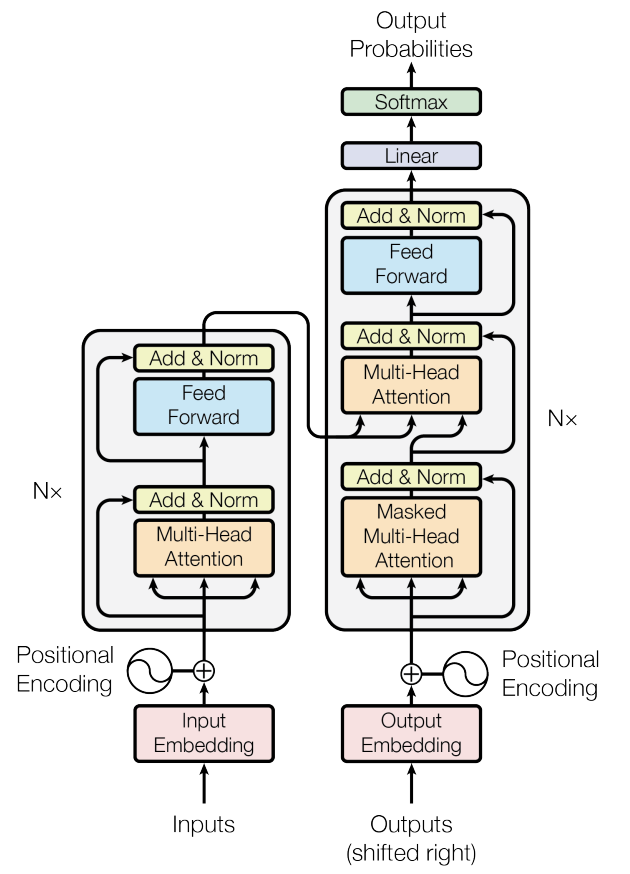
\includegraphics[width=0.6\linewidth]{figures/transformer-architecture.png}
    \caption{\textbf{The Transformer architecture}. The illustration~\cite{transformer} shows the original Transformer architecture, with both the encoder and the decoder modules, featuring the multihead-attention operator}
    \label{fig:original-transformer}
\end{figure}

Each layer in the transformer architecture contains two types of sub-modules: the multi-head attention module (see Figure \ref{fig:mha}) and the feedforward neural network. The encoder layer only has a single attention sub-module, whereas the decoder contains two, unless the model is a decoder-only model. The multi-head attention module computes a weighted average of the input sequence, where the weights are determined by the attention mechanism. The attention mechanism computes the similarity between each token in the input sequence and every other token, and uses these similarities to compute a set of attention weights. These weights are used to compute a weighted average of the input sequence, where the weights reflect the importance of each token in the sequence. The feedforward neural network applies a linear transformation to the input sequence, followed by a non-linear activation function such as ReLU. Finally, a layer normalization is applied to the output of the attention, and a residual connection is added. The transformer architecture also includes positional encoding, which allows the model to distinguish between tokens based on their position in the sequence. The positional encoding is added to the input embeddings before they are processed by the decoder.

\begin{figure}[H]
    \centering
    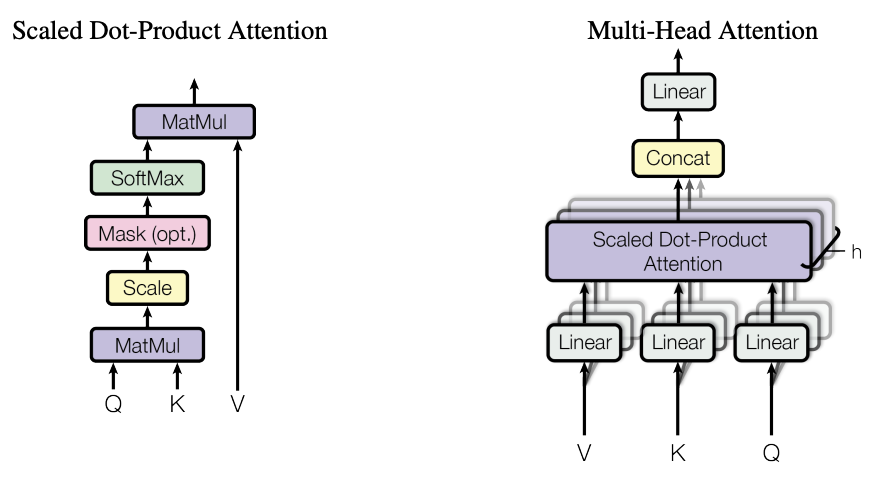
\includegraphics[width=0.6\linewidth]{figures/mha_architecture.png}
    \caption{\textbf{The Multihead Attention operator ~\cite{transformer}}}
    \label{fig:mha}
\end{figure}

\subsection{GPT models}\label{gpt-overview}
\begin{figure}[H]
    \centering
    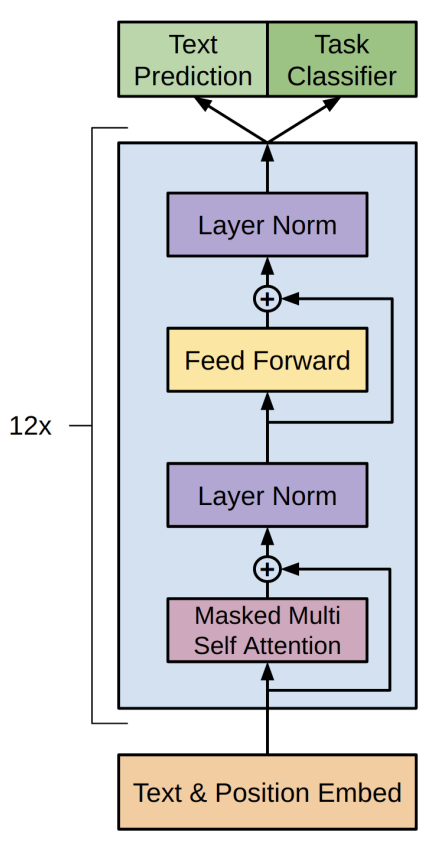
\includegraphics[width=0.3\linewidth]{figures/gpt1_architecture.png}
    \caption{\textbf{The GPT architecture}. The illustration ~\cite{gpt1} shows the original GPT architecture. GPT-2 and GPT-3 use the same architecture, with very small modifications }
    \label{fig:gpt-original}
\end{figure}
A typical GPT architecture is shown in Figure \ref{fig:gpt-original}.
The GPT architecture~\cite{gpt1, gpt2} differs from a plain Transformer architecture in a few ways. Overall, the main difference is that GPT models are decoders-only, meaning that they only employ the decoder layers from the transformer, and do not use the encoder layers. In addition to dropping the encoder layers, the GPT has the following characteristics:
\begin{itemize}
    \item \underline{Unidirectional attention}: The original Transformer architecture is bidirectional, meaning that it takes into account both past and future tokens when encoding a sequence of text. The GPT architecture, on the other hand, is unidirectional and only considers the past tokens when generating output.
    \item \underline{Causal Masking}: The original Transformer architecture is only required to use masking to prevent the model from attending to future tokens during inference, whereas the GPT architecture uses masking to prevent the model from attending to any tokens beyond the current one during both training and inference.
    \item \underline{Positional Encoding}: The GPT architecture uses a slightly different method of positional encoding compared to the original Transformer architecture. In GPT, the positional encoding is added directly to the input embeddings, whereas in the original Transformer architecture, the positional encoding is added to the output of the multi-head attention layer.
    \item \underline{Training tasks}: The pre-training objectives used for the GPT architecture are different from the original Transformer. Specifically, GPT is pre-trained using a language modeling objective, where the model is trained to predict the next token in a sequence, while the original Transformer is pre-trained using a masked language modeling objective, where the model is trained to predict masked tokens in a sequence.
\end{itemize}

Overall, the GPT architecture is a modification of the Transformer architecture, tailored specifically for language generation tasks such as text completion and dialogue generation. The differences in architecture and pre-training objectives are designed to make the model better suited to these tasks, resulting in state-of-the-art performance on a variety of natural language generation benchmarks.

\subsection{Mixture of Experts}\label{moe-layer}
A Mixture-of-Experts (MoE) layer, whose structure can be seen in Figure \ref{fig:moe-illustation}, combines a set of \textit{experts} with a \textit{gating network} (also called \textit{routing network}). Each expert is usually a feed-forward neural network (FFN), and the gating network is a function routing each input token to a sparse subset of the experts. Through training of the gating network, different experts will thus end up specializing on different subsets of the input data. The dynamic nature of the MoE architecture comes from two main sources. First, tokens are not distributed equally among experts (although MoE models tend to use loss terms to prevent excessive load imbalance) due to the use of the gating function. In Figure \ref{fig:expert_popularity}, for example, we can see how the popularity of various experts changes over the course of the training iterations. Second, in many MoE models, the \textit{capacity factor} is adjusted dynamically during training \cite{switch_transformer, tutel, dynamoe}, resulting in additional changes to the execution plan.
\begin{figure}[H]
    \centering
    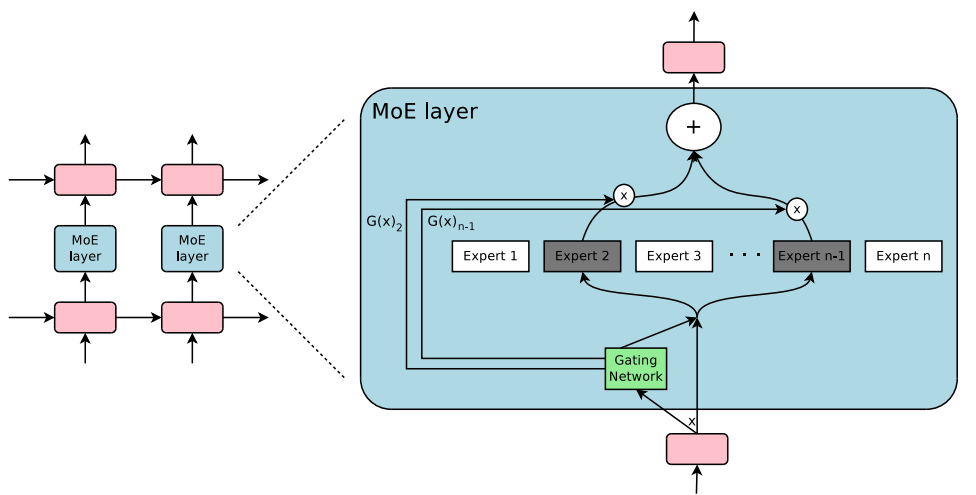
\includegraphics[width=0.6\linewidth]{figures/moe-illustration.png}
    \caption{\textbf{The Mixture of Expers (MoE) architecture}. The illustration~\cite{shazeer2017} shows a sparsely-gated MoE layer embedded within a recurrent language model.}
    \label{fig:moe-illustation}
\end{figure}


\begin{figure}[H]
    \centering
    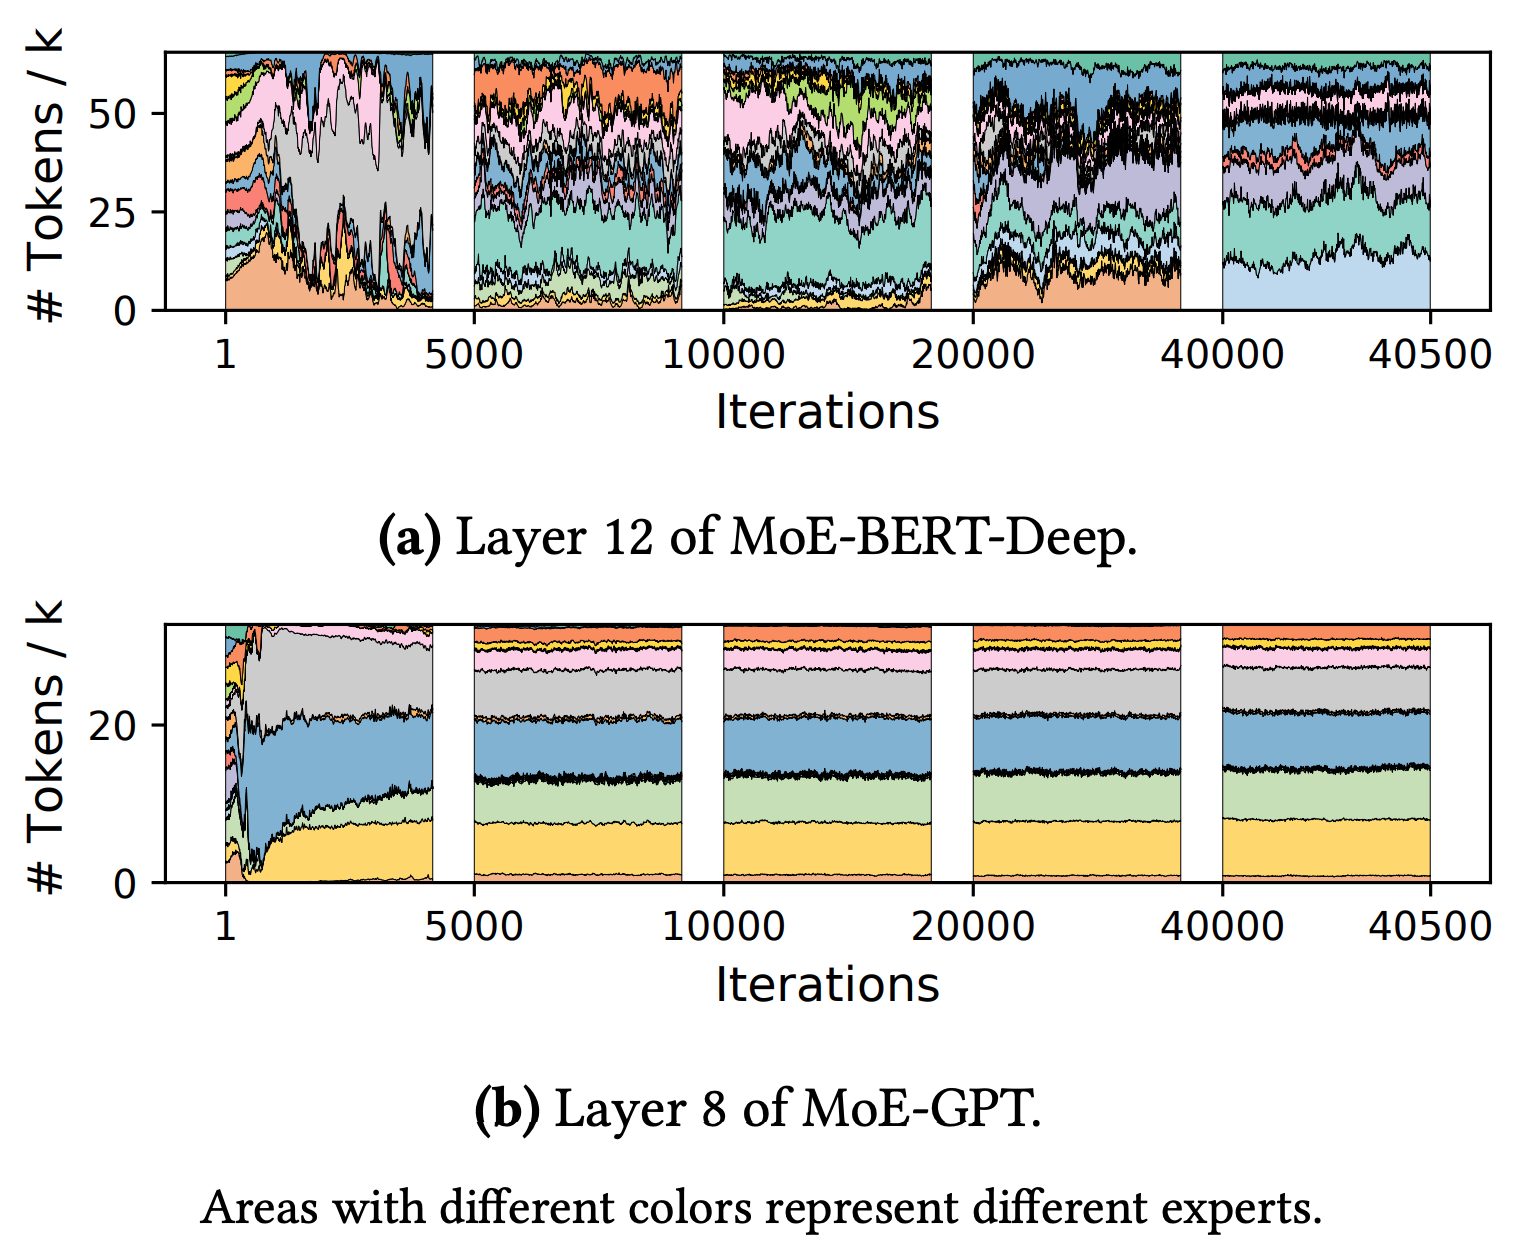
\includegraphics[width=0.6\linewidth]{figures/experts_popularity.png}
    \caption{\textbf{Load balance among experts across iterations~\cite{fastermoe}} Two models show different patterns of expert popularity over the course of training with the FasterMoE framework }
    \label{fig:expert_popularity}
\end{figure}

\subsubsection{Architecture}

A Mixture-of-Experts (MoE) layer can be defined as follows~\cite{shazeer2017}:
\begin{equation}
    y = \sum_i^n G(x)_i E_i(x)
\end{equation}

where $E_i$ is the $i$-th expert and $G(x)$ is a gating network returning a sparse $n$-dimensional vector. There can be thousands of experts, but whenever $G(X)_i=0$, we don't have to compute $E_i(x)$, since it won't be a factor in the output.

%If the number of experts is very large, we can build a two-level hierarchical MoE, and reduce the branching factor~\cite{shazeer2017}: 
%\begin{equation}
%y_H = \sum_{i=1}^a \sum_{j=1}^b G_{\text{primary}}(x)_i \cdot G_i(x)_j \cdot E_{i,j}(x)
%\end{equation}
%where we are selecting among $a$ groups of $b$ experts each by means of a primary gating network $G_{\text{primary}}$ and $a$ secondary gating networks. 

An important parameter in MoE architectures is the \textit{expert capacity}, or the batch size of each expert (the maximum number of tokens than can routed to an expert). A commonly-used formula~\cite{tutel} for the expert capacity is shown in Equation \ref{eq:expert_capacity}, where $k$ is the parameter from the top-k gating function, $T$ is the number of tokens per batch, $E$ is the number of experts, and $f$ is the \textit{capacity factor}.
\begin{equation}\label{eq:expert_capacity}
    expert\_capacity = k \cdot f \cdot \frac{T}{E}
\end{equation}
The expert capacity is usually tuned through the capacity factor, and allows us to trade between the likelihood of expert overflow (when the number of token dispatched to an expert exceeds the expert capacity) and greater computation and communication costs \cite{switch_transformer}. 


%\subsection{Token Routing}
%\subsection{Load Balancing}
%\subsection{Communication costs optimization }



\subsection{GPT-MoE}\label{gpt-moe}
The GPT model can be easily \textit{MoEfied} by substituting the Feed Forward network in the the decoder with a MoE layer. For example, the sparse models~\cite{fairseq-checkpoint} whose checkpoints are available in the Fairseq repository~\footnote{\url{https://github.com/facebookresearch/fairseq/tree/main/examples/moe_lm}} use 12 (15B-parameters model), 24 (52B- parameters and 207B-parameters models) or 32 (1.1T-parameters model) decoder layers, where every other layer contains a MoE component instead of the regular FFN. In Listing \ref{fairseq-15-moe}, we can see the 15B parameters model, where the six even-numbered decoder layers contain a FFN with two fully-connected layers, and the six odd-numbered decoder layers contain a MoE Layer instead.

\begin{lstlisting}[caption=Fairseq’s 15B-parameters MoE model, breaklines=true, basicstyle=\footnotesize, frame=single, label=fairseq-15-moe]
TransformerLanguageModel(
  (decoder): TransformerDecoder(
    (dropout_module): FairseqDropout(p=0.1)
    (embed_tokens): Embedding(50264, 768, padding_idx=1)
    (embed_positions): SinusoidalPositionalEmbedding()
    (layers): ModuleList(
      (0): TransformerDecoderLayer(
        [checkpointed]
        (dropout_module): FairseqDropout(p=0.1)
        (self_attn): MultiheadAttention(
          (dropout_module): FairseqDropout(p=0.1)
          (k_proj): Linear(in_features=768, out_features=768, bias=True)
          (v_proj): Linear(in_features=768, out_features=768, bias=True)
          (q_proj): Linear(in_features=768, out_features=768, bias=True)
          (out_proj): Linear(in_features=768, out_features=768, bias=True)
        )
        (self_attn_layer_norm): LayerNorm((768,), eps=1e-05, elementwise_affine=True)
        (activation_dropout_module): FairseqDropout(p=0.0)
        (fc1): Linear(in_features=768, out_features=3072, bias=True)
        (fc2): Linear(in_features=3072, out_features=768, bias=True)
        (final_layer_norm): LayerNorm((768,), eps=1e-05, elementwise_affine=True)
      )
      (1): TransformerDecoderLayer(
        [checkpointed]
        (dropout_module): FairseqDropout(p=0.1)
        (self_attn): MultiheadAttention(
          (dropout_module): FairseqDropout(p=0.1)
          (k_proj): Linear(in_features=768, out_features=768, bias=True)
          (v_proj): Linear(in_features=768, out_features=768, bias=True)
          (q_proj): Linear(in_features=768, out_features=768, bias=True)
          (out_proj): Linear(in_features=768, out_features=768, bias=True)
        )
        (self_attn_layer_norm): LayerNorm((768,), eps=1e-05, elementwise_affine=True)
        (moe_layer): MOELayer()
        (final_layer_norm): LayerNorm((768,), eps=1e-05, elementwise_affine=True)
      )

      ...
      
      
      (11): TransformerDecoderLayer(
        [checkpointed]
        (dropout_module): FairseqDropout(p=0.1)
        (self_attn): MultiheadAttention(
          (dropout_module): FairseqDropout(p=0.1)
          (k_proj): Linear(in_features=768, out_features=768, bias=True)
          (v_proj): Linear(in_features=768, out_features=768, bias=True)
          (q_proj): Linear(in_features=768, out_features=768, bias=True)
          (out_proj): Linear(in_features=768, out_features=768, bias=True)
        )
        (self_attn_layer_norm): LayerNorm((768,), eps=1e-05, elementwise_affine=True)
        (moe_layer): MOELayer()
        (final_layer_norm): LayerNorm((768,), eps=1e-05, elementwise_affine=True)
      )
    )
    (layer_norm): LayerNorm((768,), eps=1e-05, elementwise_affine=True)
    (output_projection): Linear(in_features=768, out_features=50264, bias=False)
  )
)
\end{lstlisting}


\section{Related Works}\label{related-works}
In this section, we introduce existing serving systems for Transformers/GPT (Section \ref{transformer-serving}) and GPT-MoE (Section \ref{chpt2-moe-serving}) models.

\subsection{Transformer serving systems}\label{transformer-serving}
There is a large number of systems that can serve transformers. In this section, we focus on the systems that are specifically optimized for transformers. These systems are also the ones that have more similar components to \Project.

\subsubsection{TurboTransformers}
TurboTransformer~\cite{turbo_transformers} is an inference system for transformers from Tencent. The system consists of two components (see Figure \ref{fig:turbo-transformers}): a serving framework, and a computational runtime.

\begin{figure}[H]
    \centering
    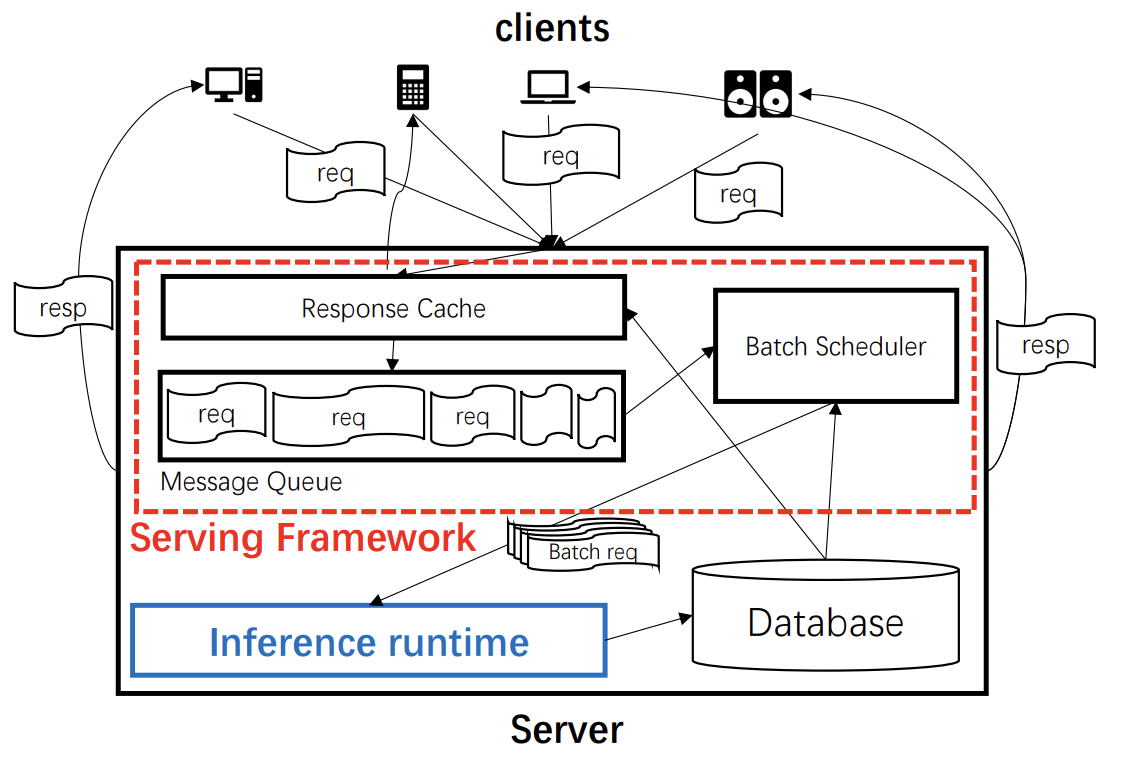
\includegraphics[width=0.6\linewidth]{figures/turbo_transformers.png}
    \caption{\textbf{The TurboTransformers system} A diagram~\cite{fastermoe} showing the components of the TurboTransformers system}
    \label{fig:turbo-transformers}
\end{figure}

The serving framework receives requests from the user via a gRPC/HTTP endpoint, and uses a dynamic programming algorithm to decide how to batch together the requests that arrive over a specific interval of time. The batch assignment considers the length of each request and attempts to minimize the amount of padding needed while also maximizing the performance gains that come from batching together as many requests as possible. 

The computational runtime takes the DNN model as input, represents it as a computational graph, and fuses all the non-GEMM kernels together. The fused computations are implemented with custom CUDA kernels that come with the TurboTransformers framework. In particular, the framework focuses on optimizing the performance of reduction kernels, such as those needed in the Softmax and LayerNorm operators. In addition to the kernel optimizations, the computational runtime also includes a custom memory manager to minimize the GPU memory overhead by reusing as much allocated memory as possible to store intermediate results. This is made possible thanks to a memory allocator that takes into consideration the topology of the computational graph to decide when to assign different tensors to the same region in memory.

The main limitations of the TurboTransformers system are the lack of support for the MoE architecture, and more importantly, the lack of support for multi-GPU and multi-node machines.


\subsubsection{FasterTransformer and Triton}
FasterTransformer~\cite{faster_transformer} is an open-source inference system by NVIDIA supporting multi-GPU execution. As the name suggests, the inference system is specialized for Transformers, and it supports a wide variety of models, including BERT~\cite{bert}, XLNet~\cite{xlnet}, GPT~\cite{gpt1, gpt2, brown_2020}, OPT~\cite{opt}, GPT-MoE, BLOOM~\cite{bloom}, GPT-J~\cite{gpt-j}, Longformer~\cite{longformer}, T5~\cite{t5}, Swin Transformer~\cite{swin-transformer}, and ViT~\cite{vit}. The FasterTransformer's backend is implemented using C++, CUDA and cuBLAS, and several front-ends are available, including C++, TensorFlow and PyTorch. The repository contains an example MoE implementation~\footnote{\url{https://github.com/NVIDIA/FasterTransformer/blob/main/docs/gpt\_guide.md\#gpt-with-moe}}, which we use in our evaluation to compare the performance of \Project with FT. 

Unlike TurboTransformers, FasterTransformer does not come with a serving framework, but NVIDIA released Triton~\cite{triton}, an open-source inference system that can be coupled with FasterTransformer via the Triton FasterTransformer Backend~\cite{triton-ft-backend}

\subsubsection{Orca}
Orca~\cite{orca} is a distributed inference system for transformers, employing optimizations such as dynamic batching and iteration-level scheduling to boost the performance of variable-length requests whose arrival times are not known in advance. Unfortunately, the Orca code is closed-source, and the authors are not planning to make it publicly available as it is being used in production by for-profit company FriendliAI, so we cannot compare the performance with our system. 

\subsection{Speculative decoding systems}
Two speculative decoding systems~\cite{speculative-decoding-berkeley, speculative-decoding-google} have been introduced in recent months. 

\section{MoE Serving Systems}\label{chpt2-moe-serving}
There are several distributed inference systems that are capable of serving MoE models. For example, FasterTransformer mentioned above, together with Fairseq~\cite{fairseq} (with additional support for the Tutel~\cite{tutel} optimizations) and Alpa~\cite{alpa}. These systems however, were designed primarily for training and do not have as many optimizations as DeepSpeed-MoE~\cite{deepspeed-moe} for the MoE inference scenario.

\subsection{DeepSpeed-MoE}
DeepSpeed-MoE~\cite{deepspeed-moe} is currently the most well-optimized distributed inference framework with best performance for serving MoE models. The optimizations behind DeepSpeed-MoE's performance can be divided in three categories: the parallelization plan (see Figure \ref{fig:deepspeed-moe-parallelization}), the hierarchical all-to-all communications (see Figure \ref{fig:deepspeed-moe-a2a}), and the use of an efficient kernel for the MoE layers.
\begin{figure}[H]
    \centering
    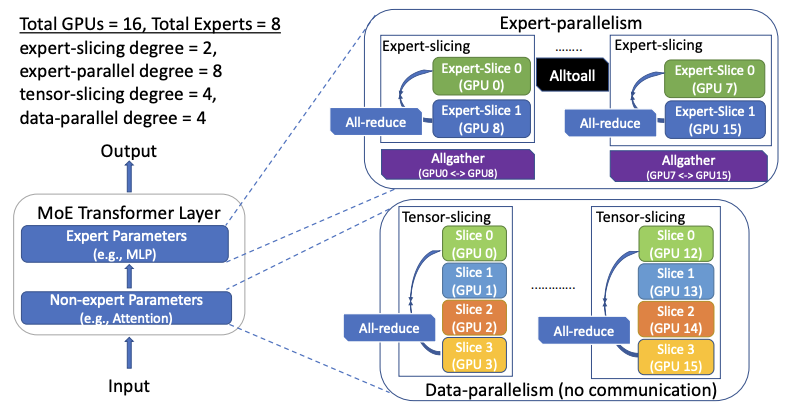
\includegraphics[width=0.6\linewidth]{figures/deepspeed-moe-parallelization.png}
    \caption{\textbf{The DeepSpeed-MoE parallelization mechanism~\cite{deepspeed-moe}}}
    \label{fig:deepspeed-moe-parallelization}
\end{figure}
DeepSpeed-MoE's parallelization plan consists of a combination of data and model parallelism. Expert layers are partitioned 
\begin{figure}[H]
    \centering
    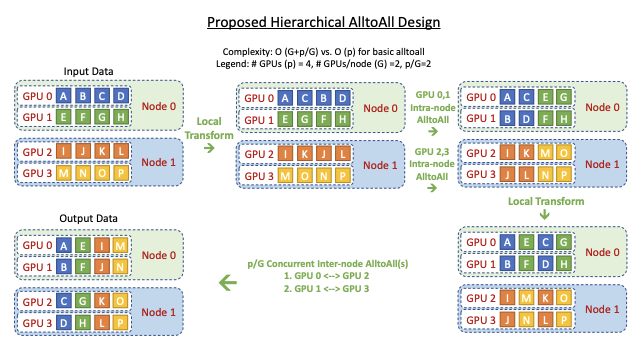
\includegraphics[width=0.6\linewidth]{figures/deepspeed-moe-a2a.png}
    \caption{\textbf{The DeepSpeed-MoE Hierarchical all-to-all design~\cite{deepspeed-moe}}}
    \label{fig:deepspeed-moe-a2a}
\end{figure}

% !TeX root = ../thuthesis-example.tex
\chapter{Design}
\section{Autoregressive inference}
\section{Parallelization}
\section{Computational graph substitutions}
\section{Communication optimizations}
\section{Kernel optimizations}

% !TeX root = ../thuthesis-example.tex

\chapter{Autoregressive transformer inference}


\section{Autoregressive transformer inference}

\section{Incremental decoding}

\section{Dynamic Batching}
% !TeX root = ../thuthesis-example.tex

\chapter{Autoregressive transformer inference}\label{chapter-5}


\section{Autoregressive transformer inference}\label{autoregressive-characterization}

A key challenge preventing transformer inference systems from achieving low latency is the \textit{autoregressive} nature of many generative tasks of interest, such as sentence completion, language modeling or machine translation. By "autoregressive" we mean that in these tasks, each generated token depends on all those preceding it. This dependency is required, otherwise the model will simply output a sequence of unrelated words. As a consequence, we need to generate each token sequentially, and feed it back to the model to generate the following token in the following iteration. Some existing works have tried to push the performance by performing inference in a non-autoregressive fashion, by relaxing the assumption of conditional dependence of tokens on the preceding ones, but these techniques have so far been unable to match the quality of the output of their autoregressive counterparts, without increasing the computational costs.  

Unlike these previous approaches, in ExpertFlow we employ three key components to support conditionally-dependent token generation while at the same time significantly reducing the overhead of serial generation. The three components are orthogonal and can be independently applied to improve the performance. This chapter focuses on these three optimizations, which are discussed in the sections below.

\section{Dynamic Batching}\label{dynamic-batching}
In both training and inference, batching multiple input sequences together is essential to maximize the device utilization, thus optimizing the throughput. Batching, however, can also be a source of inefficiency. First of all, if the requests in a batch do not all have the same length, we have to pad them to the maximum sequence length, resulting in wasted computations. In the inference case, additional challenges are that we may not be able to fill an entire batch with requests, as requests are not all available in advance, and we don't know when they will arrive. This requires more padding, and more wasted computations. Finally, and most importantly, because of the autoregressive nature of many transformers models, inference requires one iteration for each token to be generated. Since the requests in a single batch may have different final lengths, and we need to run the model once for each token to be generated, we will need to run the model on the batch a number of times equal to the maximum number of tokens to be generated, across all requests in the batch. This will require a large amount of computations, since the inference stage for all requests with a lower number of tokens to be generated will have already completed. In addition, the requests that have already completed will have to wait for the straggler request to complete before the result can be returned to the client, resulting in a large latency overhead.

In ExpertFlow, we use a dynamic batching design to reap the benefits of batching (increased device utilization), while keeping the overhead caused by the disuniform sequence lengths and arrival times to a minimum. We do that through the following steps:
\begin{enumerate}
    \item Merge the sequence and batch dimensions together, effectively treating the tokens from the batch's request as a single sequence. This allows us to store all the tokens in contiguous memory, avoiding the need for padding each request to the maximum sequence length. To keep all tensors of the same size, we will still need to pad the flattened sequence to $batch\_size \cdot max\_seq\_len$, but leaving all the padding in contiguous memory after the tokens. As the padding is no longer fragmented between the requests, we can avoid unnecessary computations by sending the token count to the model's operator, so they can simply skip over the last $token\_embedding\_dim \cdot ((batch\_size \cdot max\_seq\_len) - token\_count)$ entries in the tensor.
    \item We update the batch at each generative step, instead of waiting for all the requests to be completed. 
    \item We attach some metadata to each batch, to facilitate steps 1 and 2. This is especially important for operators such as the attention, which needs to know what sequence each tokens belongs to, and at what position it is located. We use the \texttt{BatchConfig} struct in Listing \ref{batchConfigListing}.
\end{enumerate}

\begin{lstlisting}[language=C++, caption=BatchConfig, breaklines=true, basicstyle=\footnotesize, frame=single, label=batchConfigListing]
class BatchConfig {
public:
  BatchConfig();
  bool register_new_request(size_t guid,
                            int initial_length,
                            int tokens_to_generate);
  void prepare_next_batch();
  int update_results(InferenceResult const &ir);
  void update_num_active_requests_tokens();
  int num_active_requests() const;
  int num_active_tokens() const;
  void print() const;
  static int const MAX_NUM_REQUESTS = MAX_REQUESTS;
  static int const MAX_NUM_TOKENS = InferenceResult::MAX_NUM_TOKENS;
  // static int const MAX_SEQUENCE_LENGTH = MAX_SEQ_LEN;
  //  These are set by update
  int num_tokens, num_requests;
  bool cached_results;
  int token_start_idx[MAX_NUM_REQUESTS]; // index of first token in a request
                                         // that should be processed in the
                                         // current batch/iteration
  int token_last_available_idx
      [MAX_NUM_REQUESTS]; // last valid token index in a request. This includes
                          // both the prompt and generated tokens
  int num_processing_tokens[MAX_NUM_REQUESTS]; // a request's number of tokens
                                               // being processed in the current
                                               // batch/iteration
  size_t max_sequence_length[MAX_NUM_REQUESTS];

  struct token_idxs {
    size_t request_index;  // the index within the BatchConfig of the request
                           // that the token belongs to
    size_t token_position; // the index indicating the position of each token
                           // within its request
  };

  struct SampleIdxs {
    size_t num_samples;
    size_t guids[InferenceResult::MAX_NUM_TOKENS]; // the guid of the request
                                                   // each token belongs to
    token_idxs token_indexes[InferenceResult::MAX_NUM_TOKENS];
  };

  SampleIdxs token2ids;
  size_t request_guid[MAX_NUM_REQUESTS];
  bool request_completed[MAX_NUM_REQUESTS];
};
\end{lstlisting}

\section{Incremental decoding}\label{incr-decoding-section}
Similarly to other existing transformer systems~\cite{fairseq, orca}, we employ incremental decoding to eliminate the redundant computations that would otherwise be needed when generating tokens in a autoregressive fashion. To understand why autoregressive decoding will engender redundant computations (in the absence of incremental decoding), we have to look at how the multi-head attention operator works (see Algorithm \ref{alg:attn}). 
\begin{algorithm}[H]
  \caption{Multi-Head Self-Attention algorithm}
  \label{alg:attn}
  \small
  \begin{algorithmic}[1]
    \Ensure $x$: input sequence, $W_{qkv}$: Q/K/V projection weights, $W_{o}$: output projection weights, $num\_heads$: number of attention heads,  $seq\_len$: maximum number of tokens in each request, $batch\_size$: number of requests in each batch, $emb\_dim$: embedding dimension
    \Require shape of $x = [emb\_dim, seq\_len, batch\_size]$
    \Require shape of $W_{qkv} = [emb\_dim, Q\_proj + K\_proj + V\_proj, num\_heads]$
    \Require shape of $W_{o} = [V\_proj \times num\_heads, emb\_dim]$
    \State $QKV\_projs \leftarrow W_{qkv}^Tx$
    \State $Q \leftarrow QKV\_projs \; [\; : \;, \; : Q\_proj, \; : \;]$  
        \Comment{Shape : $(num\_heads, Q\_proj, seq\_len, batch\_size)$}
    \State $K \leftarrow QKV\_projs \; [\; : \;, \; Q\_proj : Q\_proj + K\_proj, \; : \;]$ 
        \Comment{Shape : $(\dots, K\_proj, \dots)$}
    \State $V \leftarrow QKV\_projs \; [\; : \;, \; Q\_proj + K\_proj : \;, \; : \;]$ 
        \Comment{Shape : $(\dots, V\_proj, \dots)$}
    \State $QK^T \leftarrow einsum("ijkl,ijmn\rightarrow klmni",Q,K)$ 
        \Comment{Shape : $(seq\_len, batch\_size, seq\_len, batch\_size, num\_heads)$}
    \State $QK^T \leftarrow CausalMasking(QK^T)$
        \Comment{Set entries above diagonal to $-\infty$}
    \State $attn \leftarrow softmax(\frac{QK^T}{\sqrt{K\_proj}})$
    \State $attn \leftarrow einsum("ijklm,mnkl \rightarrow ijnm", attn, V)$
        \Comment{Shape : $(seq\_len, batch\_size, V\_proj, num\_heads)$}
    \State $attn \leftarrow attn.reshape(seq\_len, batch\_size, V\_proj \times num\_heads)$
    \State $output \leftarrow (attn \times W_{o}).transpose(-1,0,1)$
        \Comment{Shape : $(emb\_dim, seq\_len, batch\_size)$}
  \end{algorithmic}
\end{algorithm}
In the decoding case, given an input sequence $x$, we will first generate the $Q_h$, $K_h$ and $V_h$ projections by matrix multiplying $x$ by the weight matrices $W_h^Q$, $W_h^K$ and $W_h^V$, for each head $h$:
\begin{align}\label{qkv-equations}
    Q_h = (W_h^Q)^\top x \\
    K_h = (W_h^K)^\top x \\
    V_h = (W_h^V)^\top x \\
\end{align}
Then, for each head, we compute the attention scores with the formula:
\begin{equation}\label{attn-formula}
    Attention(Q_h, K_h, V_h) = softmax\left(\frac{Q_h \times K_h^\top}{\sqrt{d_k}}\right) \times V_h
\end{equation}
where $d_k$ is the dimension of the $Q_h$ and $K_h$ arrays. The output of the multi-head attention layer is then obtained by concatenating the results of Equation \ref{attn-formula} for all heads, and performing one more matrix multiplication to project the result in the output space: 
\begin{equation}
    Output = Concat(\{Attention(Q_h, K_h, V_h) \;\; \forall h \in [0, num\_heads-1]\}) \times W_{out}
\end{equation}
The length of the output tensor is equal to the length of each $Q_h$ projection, which is in turn equal to the length of $x$. This can help us understand where the redundant computations come from. In fact, at the end of each iteration, we only save the output in the last token's slot, and discard all outputs in the preceding slots, as these will be unchanged from the previous iterations. 

Incremental decoding works by computing $Q_h$ using only the last entry of $x$, so the output will also have only one entry, which is all that we need. In a model with only one attention layer, changing Equation \ref{qkv-equations} to Equation \ref{q_proj_one_element} below would be enough.
\begin{equation}\label{q_proj_one_element}
    Q_h = (W_h^Q)^\top x[ : -1] \\
\end{equation}
This would compute the attention scores with respect to all preceding tokens (as we would still be using the full $x$ array to compute $K_h$ and $V_h$), but only output the result for the last token. We would then pass only one output to the following layers, thus saving a lot of unnecessary computations. However, in the scenario where the model contains multiple attention layers (as is usually the case), our optimization doesn't work, because after the first attention, all the following attention layers only receive one entry (the one corresponding to the last token), which is enough to compute $Q_h$, but not enough to compute $K_h$ and $V_h$. Incremental decoding fixes this problem by letting each attention operator cache the Key ($K_h$) and Value ($V_h$) projections. This solution works because at each iteration, and in each attention layer, only the last entry of ($K_h$) and ($V_h$) is changed. Note that this is only the case after having processed the prompt, which will still require passing all the tokens to the model, so that we can initialize the Key and Value entries in the cache for all tokens in the prompt. For more details on how incremental decoding works, see Algorithm \ref{alg:attn2}.
\begin{algorithm}[H]
  \caption{Multi-Head Self-Attention with Incremental Decoding}
  \label{alg:attn2}
  \small
  \begin{algorithmic}[1]
    \Ensure $x$: input sequence, $W_{qkv}$: Q/K/V projection weights, $W_{o}$: output projection weights, $K\_cache$ \& $V\_cache$: the K/V projections for the previous tokens in all in-progress requests, $num\_heads$: number of attention heads, $batch\_config$: the \texttt{BatchConfig} object with the batch's metadata
    \Require shape of $x$ = [emb\_dim, batch\_config.num\_tokens]
    \Require shape of $W_{qkv}$ = [emb\_dim, Q\_proj + K\_proj + V\_proj, num\_heads]
    \Require shape of $W_{o}$ = [V\_proj \times num\_heads, emb\_dim]
    \Require shape of $K\_cache$ = [K\_proj, max\_seq\_len, num\_heads, max\_requests]
    \Require shape of $V\_cache$ = [V\_proj, max\_seq\_len, num\_heads, max\_requests]
    \State $QKV\_projs \leftarrow W_{qkv}^Tx$
    \State Q $\leftarrow$ QKV\_projs [ : , : Q\_proj, : ]
        \Comment{Shape : (num\_heads, Q\_proj, batch\_config.num\_tokens)}
    \State K $\leftarrow$ QKV\_projs [ : , Q\_proj : Q\_proj + K\_proj, : ]
        \Comment{Shape : ($\dots$, K\_proj, $\dots$)}
    \State V $\leftarrow$ QKV\_projs  [ : , Q\_proj + K\_proj : , : ]
        \Comment{Shape : ($\dots$, V\_proj, $\dots$)}
    \State processed\_tokens $\leftarrow 0$
    \State attn $\leftarrow []$
    \For{$r$}{$1$}{$batch\_config.num\_requests$}
        \State $l_r \leftarrow$ current length of request $r$
        \State $n_r \leftarrow$ number of new tokens from request $r$ in this batch
        \State Store new $K$ projection in K\_cache[ : , $l_r$ : $l_r + n_r$, : , r ]
        \State Store new $V$ projection in V\_cache[ : , $l_r$ : $l_r + n_r$, : , r ]
        \State $QK^T_r \leftarrow$ einsum($"ijk,jli\rightarrow kli"$, Q [ : , : , processed\_tokens : processed\_tokens + $n_r$ ], K\_cache[ : , : $l_r + n_r$ , : , r])
            \Comment{Shape : ($n_r$, $l_r + n_r$, num\_heads)}
        \State $QK^T_r \leftarrow CausalMasking(QK^T_r)$
            \Comment{Set entries above diagonal to $-\infty$}
        \State $attn_r \leftarrow softmax\left(\frac{QK^T_r}{\sqrt{K\_proj}}\right)$
        \State $attn_r \leftarrow$ einsum($"ijk,ljk \rightarrow ilk"$, $attn_r$, V\_cache[ : , : $l_r + n_r$ , : , r])
            \Comment{Shape : ($n_r$, V\_proj, num\_heads)}
        \State attn $\leftarrow$ concatenate (attn, $attn_r$)
        \State processed\_tokens $\leftarrow processed\_tokens + n_r$
    \EndFor
    \State $attn \leftarrow attn.reshape(batch\_config.num\_tokens, V\_proj \times num\_heads)$
    \State $output \leftarrow (attn \times W_{o}).transpose(-1,0,1)$
        \Comment{Shape : $(emb\_dim, batch\_config.num\_tokens)$}
  \end{algorithmic}
\end{algorithm}

Having formalized how incremental decoding works, we can now quantify the amount of redundant computations saved by this technique. To do so, we develop a simple model (see below) to estimate the total number of floating point operations (FLOPs) required by one iteration of the multi-head attention operator in one layer, both before (Algorithm \ref{alg:attn}) and after (Algorithm \ref{alg:attn2}) adopting incremental decoding. We can then compute the difference between these two quantities, and we will now the number of FLOPs saved at each attention layer. The total number of FLOPs saved by the entire model will be much higher, as every layer (not just the attention layers) will be able to only process a single token per iteration (after the first iteration, where we need to pass the full prompt to the model). Computing the total number of FLOPs saved in the general case is not possible, since it depends on the exact structure of the model. However, if we are given a specific model, we can estimate the number of FLOPs required by each layer as a function of the sequence length, and then compute the number of FLOPs saved, in the same way as we do below for the attention layer.

Let's now estimate the FLOPs required by Algorithm \ref{alg:attn} and Algorithm \ref{alg:attn2}. Before we begin, however, we need to make an assumption regarding the FLOPs required by matrix multiplication and the softmax operator.  For the matrix multiplication, we assume that we will be using the naive matrix multiplication algorithm, which will require $2xyz$ FLOPs to multiply together matrix $A\in \mathbb{R}^{x \times y}$ and $B\in \mathbb{R}^{y \times z}$. For the softmax operator, we assume that, given the same matrix $A$ that we just mentioned, the number of FLOPs to compute the result will be $3xy$. 

For Algorithm \ref{alg:attn}, we will need the following number of FLOPs:
\begin{align}
    \text{TOTAL FLOPs} = \; & 2 h (d_k + d_k + d_v) d_m \cdot (l \cdot b) + \\
    & 2 h d_k (l \cdot b)^2 + \\
    & h \cdot (l \cdot b)^2 + \\
    & 3h(l \cdot b)^2 + \\
    & 2h (l \cdot b)^2 \cdot d_v + \\
    & 2h(l \cdot b) d_v d_m
\end{align}
where we have used the following notation: $h$ is the number of heads, $d_k$ is the dimension of each Query and Key projection (which must be equal), $d_v$ is the dimension of each Value projection, $d_m$ is the hidden dimension of the model, $l$ is the sequence length, and $b$ is the batch size. When the key and value projections have the same dimensions (i.e. $d_k = d_v$), we can simplify the expression above as follows:
\begin{equation}
    \text{TOTAL FLOPs} = 4h (l \cdot b)(2 d_k d_m + (d_k + 1) (l \cdot b))
\end{equation}
Hence, for a single request of length $l$, the number of FLOPs will be:
\begin{equation}\label{final-eq-old}
    \text{FLOPS (1 request)} = 4 h l (l + d_k (2 d_m + l))
\end{equation}

For Algorithm \ref{alg:attn2}, we will need the following number of FLOPs:
\begin{align}
    \text{TOTAL FLOPs} = \; & 2 h (d_k + d_k + d_v) d_m \cdot \sum_r n_r + \\
    & 2 h d_k \left(\sum_r n_r \cdot \sum_r l_r \right) + \\
    & h \cdot \left(\sum_r n_r \cdot \sum_r l_r \right) + \\
    & 3h\left(\sum_r n_r \cdot \sum_r l_r \right) + \\
    & 2h \left(\sum_r n_r \cdot \sum_r l_r \right) \cdot d_v + \\
    & 2h\left(\sum_r n_r \right) d_v d_m
\end{align}
where we have introduced the following additional notation: $r$ is the request index, $n_r$ is the number of new tokens from request $r$ in the current iteration ($n_r$ will be equal to the prompt length at iteration $0$, and then $n_r=1$ for all following iterations), and $l_r$ is the current length of request $r$: this quantity will always equal $n_r$ plus all the tokens previously generated for request $r$.
Just like we did above, we can then simplify the formula above as follows:
\begin{equation}
    \text{TOTAL FLOPs} = 2 h \left(\sum_r n_r \right) \left(2 d_m d_v + \left(2 + d_v \right) \left(\sum_r l_r \right) + d_k \left(2 d_m + \left(\sum_r l_r \right) \right)\right)
\end{equation}
which simplifies further when $d_v = d_k$:
\begin{equation}
    \text{TOTAL FLOPs} = 4 h \left(\sum_r n_r \right) \left( \left(\sum_r l_r \right) + d_k \left(2 d_m + \left(\sum_r l_r \right) \right)\right)
\end{equation}
For a single request, at the iteration where the total length is $l$ and the number of new tokens is $n$, the formula above simplifies to:
\begin{equation}\label{flops-incremental-two-vars}
    \text{FLOPs (1 request)} = 4 h n \left( l + d_k \left(2 d_m + l \right)\right)
\end{equation}
We can also rewrite Equation \ref{flops-incremental-two-vars} in terms of only variable $l$, for the case where the number of new tokens is always $1$ in the incremental phase:
\begin{equation}\label{final-eq-new}
    \text{FLOPs (1 request)} = \begin{cases}
                              4 h \left( l + d_k \left(2 d_m + l \right)\right)  & \text{ incremental phase} \\
                              4 h l \left( l + d_k \left(2 d_m + l \right)\right) & \text{ prompt}
\end{cases}
\end{equation}
Given a single request with a prompt length of $l_i$ and final length of $l_f$, we can now compute the number of FLOPs saved by incremental decoding with the formula below, where we let $\phi(l)$ be the number of FLOPs for a request of length $l$ at the current iteration as computed by Equation \ref{final-eq-new}, and $\psi(l)$ be the number of FLOPs for a request of length $l$ at the current iteration as computed by Equation \ref{final-eq-old}. In other words, $\phi(l)$ is the relevant equation when incremental decoding is active, and $\psi(l)$ is the equation to be used when we are not using incremental decoding. The number of FLOPs saved can then be computed as follows:
\begin{equation}
    \text{FLOPs saved} = \sum_{l=l_i}^{l_f}  \phi(l) - \sum_{l=l_i}^{l_f}  \psi(l)
\end{equation}
which expands to:
\begin{equation}
\begin{aligned}
\text{FLOPs saved} &= 4 h l_i \left( l_i + d_k \left(2 d_m + l_i \right)\right) + \sum_{l=l_i+1}^{l_f} \left( 4 h \left( l + d_k \left(2 d_m + l \right)\right) \right) - \\
&+ \sum_{l=l_i}^{l_f} \left( 4 h l (l + d_k (2 d_m + l)) \right )
\end{aligned}
\end{equation}
We can then solve with respect to $l_i$ and $l_f$, and obtain:
\begin{equation}\label{eq-closed-form}
\boxed{\begin{aligned}
    \text{FLOPs saved} = \frac{4}{3} h (l_f-l_i) (d_k \left(3 d_m (l_f+l_i+3)+l_f^2+l_f (l_i+3)+l_i^2+3l_i+2\right)+ \\
   +l_f^2+l_f (l_i+3)+l_i^2+3l_i+2)
\end{aligned}}
\end{equation}
We can see that Equation \ref{eq-closed-form} always evaluates to a positive, non-zero number. To have a more concrete idea of the number of FLOPs saved, we can plug in some example values for $l_i$ and $l_f$. For instance, assume that the prompt has a length of 32 tokens ($l_i=32$), and we want to generate 96 additional tokens ($l_f = l_i + 96 = 128$). Plugging these values into Eq. \ref{eq-closed-form} yields:
\begin{equation}
    \text{FLOPs saved} = 128 (21986 + d_k (21986 + 489 d_m)) h
\end{equation}

Finally, it is worth mentioning that for \underline{batches with more than 1 request}, Algorithm \ref{alg:attn2} will allow us to save a number of FLOPs that is \textbf{much larger} than the sum of the values obtained with formula \ref{eq-closed-form} for each request. In fact, in the absence of incremental decoding, Algorithm \ref{alg:attn} needs to pad all requests to the same maximum length, whereas Algorithm \ref{alg:attn2} does not require any padding, as it can integrate the dynamic batching optimizations discussed in Section \ref{dynamic-batching}. 

\section{Speculative decoding}\label{spec-decoding-section}

While incremental decoding already allows us to greatly reduce the multi-head attention's overhead, the generation of the tokens is still sequential, resulting in high latency compared to running the same type of model in a non-autoregressive mode. To further improve the performance, we use speculative inference.

Speculative inference allow us to decrease the latency, as well as the GPU memory accesses, which can often become a bottleneck. When it comes to the end-to-end latency, we have already discusses in Section \ref{design-speculative-inference} how the use of speculative inference can reduce the overhead by up to the average matching rate, or the average number of tokens tha the speculators can guess correctly. 

In addition to the latency improvements, the reduction in the number of times we use the larger LLM model will reduce the GPU memory accesses needed to load the weights from CPU DRAM. This will result in further speedups, since memory accesses are often the bottleneck when it comes to GPU programs. This is especially the case when we offload some of the data and computations to CPU or flash storage. 

%We load two sizes of the target model, a smaller one, and a larger one, with a number of parameters 10x larger than the smaller one. For each request, we first route the tokens to the small model, which runs in autoregressive fashion. Due to the smaller size, the latency of generation is greatly reduced. When we have reason to believe that the smaller model might be making a wrong prediction, we let the larger model run instead. The larger model will then take as input all the tokens generated so far, and compute the prediction scores for each such tokens. If all of the predictions from the larger models are close enough to the predictions from the small model, the large model will output its prediction for an additional token and then hand back control to the smaller model. On the other hand, if the prediction for one of the generated tokens is too different from the score obtained by the larger model, we replace that token with the one predicted by the larger model and discard all the following tokens. Then, we also hand back control to the smaller model.

\section{Conclusion}
In this chapter, we focused on the optimizations we employed to tackle the challenges that come with serving generative models in autoregressive mode. In Section \ref{autoregressive-characterization} we first characterized the problem. In the following three sections, we discussed the three main optimizations in ExpertFlow: dynamic batching (Section \ref{dynamic-batching}), incremental decoding (\ref{incr-decoding-section}), and speculative decoding (\ref{spec-decoding-section}). 
% !TeX root = ../thuthesis-example.tex

\chapter{Computational Graph Substitutions}

\section{Placeholder 1}

\section{Placeholder 2}

\section{Placeholder 3}


% !TeX root = ../thuthesis-example.tex

\chapter{Evaluation}\label{chapter-7}
In this section, we describe our efforts to evaluate the correctness and the performance of ExpertFlow. Evaluating the correctness amounts to ensuring that our system always produces the expected results, so that users can be confident that using ExpertFlow instead of another existing system will not result in obtaining wrong or low quality output tokens. Evaluating the performance allows us to check that ExpertFlow is faster or at least comparable to existing solutions.

\section{Evaluating correctness}\label{eval-correctness}
We evaluate the correctness of ExpertFlow through a combination of unit tests and integration-tests.

\subsection{Unit tests}
ExpertFlow inherits from FlexFlow~\cite{flexflow,unity}, the three levels of abstractions used to represent a DNN and execute its computations: \textit{layers}, \textit{operators}, and \textit{asynchronous tasks}, which in turn execute one (or more) \textit{kernel} on GPU. At each level of abstraction, we add multiple unit tests to verify the correctness under many different angles. For instance, at the layer level, we can most easily check the correctness of the structure of the model. At the operator level, we concentrate most tests that check the generated computational graph, the dimensions of the input and output tensors, and the parallelization strategies. At the task level, we can most easily check that the input and weights tensors are accessible, on the right device, and contain the correct data. Further, we can check the correctness of the GPU kernels. 

We implement our unit tests, organized as described above, using different programming languages and frameworks. At the layer, and operator level, we added tests in the form of assertions, based on quantities computed in C++, often based on the Legion library. We also used the DOT language, together with GraphViz, to export and visualize graph-structured quantities, such as the computational graphs, or the data and temporal dependencies between different tensors, operators, and tasks. Finally, we verified the correctness of all the custom kernels by re-implementing them using C++ and LibTorch (the PyTorch C++ API), running the CUDA and C++ versions in parallel, and verifying that the output tensors match. For the kernels that have a corresponding operator in PyTorch (e.g. the Linear layer, Softmax layer, LayerNorm, etc...), we also created a suite of \textit{alignment tests}, where we compare the output tensors of our kernels against the results obtained with PyTorch for a range of different input tensors. We added the alignment tests to CI, to ensure that we do not accidentally introduce new bugs with new commits.

\subsection{End-to-End tests}
After having tested each component individually, we used end-to-end tests as an additional check on the correctness of our implementation. We achieved this by choosing three representative models for which the pre-trained checkpoints is available, loading the weights into ExpertFlow, executing the same batch of inference requests using the original code and the ExpertFlow code representing the same model, and ensuring that the outputs match. In addition to loading the weights, we also needed to ensure that all the random seeds matched, whenever there was an operator with a stochastic behavior. The models we chose for this test were:
\begin{enumerate}
    \item LLAMA model~\cite{touvron2023llama} by Meta, a transformer model
    \item Fairseq’s 15B-parameters LM MoE model~\cite{fairseq-moe-model}, also by Meta, a MoE model
    \item GPT-MoE中文67亿诗歌生成模型~\cite{modelscope-checkpoint} by Modelscope, a MoE model
\end{enumerate}

\section{Evaluating performance}\label{eval-performance}
After evaluating the correctness of our framework, we ran several experiments to measure its performance. In the sections below, we discuss our experiment setup, and we present our results.

\subsection{Setup}
We run the experiments on a \texttt{g4dn.12xlarge} AWS machine with 48 vCPUs, 192 GiB of RAM memory, and 4 NVIDIA T4 GPUs (see Figure \ref{fig:gpu-setup}), each with 16 GB of memory (although the amount of usable memory is somewhat less). We initialize the instance with the Deep Learning AMI GPU PyTorch 1.13.0 (Ubuntu 20.04) 20221109. We run the FasterTransformer experiments within the \texttt{nvcr.io/nvidia/pytorch:22.07-py3} container, which comes with PyTorch built from source to add support for MPI, which is required by FasterTransformer to support the multi-GPU GPT program.

\begin{figure}[H]
    \centering
    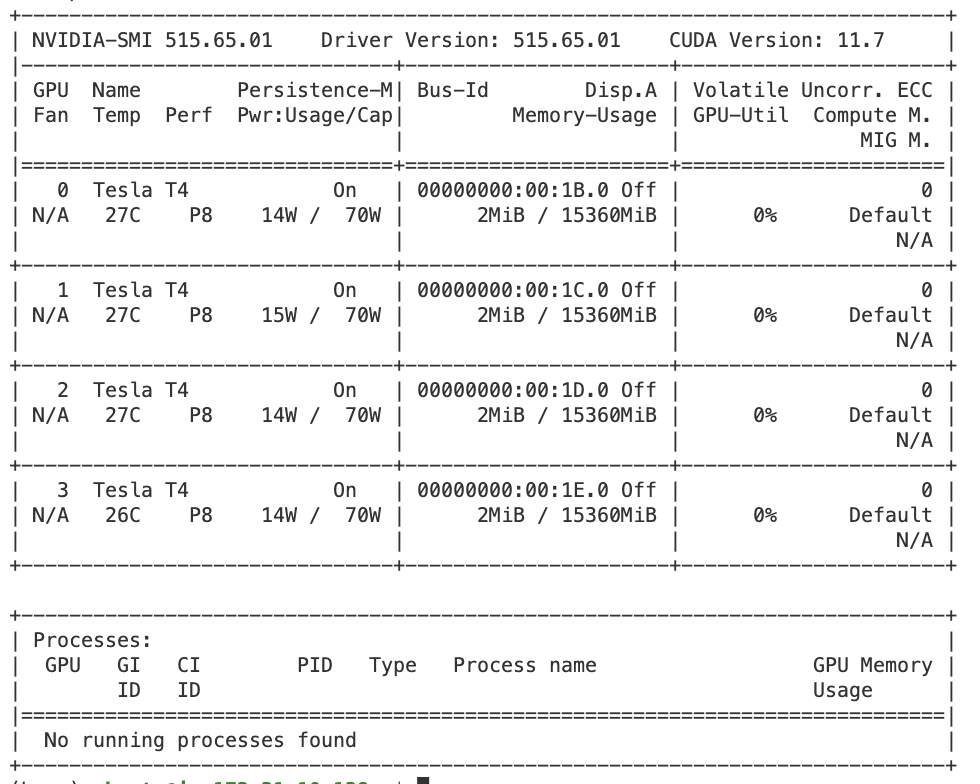
\includegraphics[width=\linewidth]{figures/nvidia-smi.png}
    \caption{\textbf{The GPU setup}}
    \label{fig:gpu-setup}
\end{figure}

\subsection{GPT-MoE model}
We ran our performance evaluation using the GPT-MoE model from Modelscope. We picked this model because it has full compatibility with FasterTransformer~\cite{faster_transformer}, as well as DeepSpeed~\cite{deepspeed-moe}, and the instructions for running it~\footnote{\url{https://github.com/NVIDIA/FasterTransformer/blob/main/docs/gpt\_guide.md\#gpt-with-moe}} in FasterTransformer are available in the GPT guide from the FasterTransformer Github repository. We use the provided scripts~\footnote{\url{https://github.com/NVIDIA/FasterTransformer/blob/main/examples/pytorch/gpt/utils/megatron\_gpt\_moe\_ckpt\_convert.py}} for converting the Modelscope checkpoint, which was built based on the Megatron-LM~\cite{megatron-lm} model specifications, to a format compatible with DeepSpeed and FasterTransformer. We then write our own custom scripts to convert and load the data into ExpertFlow.

The Modelscope MoE model is a fairly typical GPT-MoE model with 24 layers, half of which are regular FFN layers, and the other half are MoE. In particular, the odd-numbered layers are MoE. Regular FFN layers contain two dense layers, with an internal hidden dimension of size $4 \times$ as large as the hidden size. Each expert in the MoE layer also consists of two dense layers with an internal hidden dimension of size $4 \times$ as large as the hidden size. Additional settings are passed to the runtime via a human-readable \texttt{config.ini} file, whose contents are shown below (Listing \ref{config-ini}):

\begin{lstlisting}[language=Python, caption=config.ini, breaklines=true, basicstyle=\footnotesize, frame=single, label=config-ini]
[gpt]
model_name = gpt
head_num = 16
size_per_head = 64
inter_size = 4096
num_layer = 24
max_pos_seq_len = 2048
vocab_size = 51200
has_adapters = False
adapter_inter_size = 0
layernorm_eps = 1e-05
start_id = 50256
end_id = 50256
weight_data_type = fp16
tensor_para_size = 4

[structure]
gpt_with_moe = 1
expert_num = 64
moe_layers = [1, 3, 5, 7, 9, 11, 13, 15, 17, 19, 21, 23]
\end{lstlisting}


\subsection{Experiments}
\subsubsection{Workload generation}
The results of our experiments are shown below. We compare the performance of ExpertFlow to FasterTransformer, and report the throughput and latencies under different loads. We model the request arrivals using artificial traces where the arrival times are modeled by a Poisson process, and the request lengths follow a uniform distribution. This technique is similar to the approach taken in Orca~\cite{orca}. We build a workload generator that takes as input the following parameters:
\begin{itemize}
    \item the average requet arrival rate ($\lambda$)
    \item the total number of requests ($N$)
    \item the minimum ($p_{min}$) and maximum length ($p_{max}$) of the prompt
    \item the minimum ($g_{min}$) and maximum number ($g_{max}$) of tokens to generate
\end{itemize}
Given the values of the parameters above, our generator works as follows. For each request $k$, it generate the request's arrival time ($t_k$) by sampling from the Erlang distribution:
\begin{equation}
    T=\{t_1,..., T_N\} \sim Erlang(k, \lambda)
\end{equation}
The PDF of the Erlang distribution is as follows: 
\begin{equation}
    p_{T_k} = P(T_k=t)=\frac{\lambda^kt^{k-1}e^{-\lambda t}}{(k-1)!}
\end{equation}
From an implementation standpoint, we can simulate each request arrival time $t_k$, using just a uniform random number generator and the following formula: 
\begin{equation}
    t_k=-(1/k)\sum_{i=1}^k\log{u_i}
\end{equation}
where $u_i$ is the $i$-th random number generated from the uniform distribution 
\begin{equation}
    U \sim Uniform([0,1])
\end{equation}
Next, the number of tokens in the prompt $p_k$ and the number of tokens to generate ($g_k$) as output in each request are determined by sampling from the following uniform distributions:
\begin{align}
    p_k & \sim Uniform([p_{min}, p_{max}]) \\
    g_k & \sim Uniform([g_{min}, g_{max}])
\end{align}
Given the value of $p_k$, we generate the request's prompt by randomly sampling $p_k$ values from the range of integers $[0, vocab\_size -1]$.
In summary, each request $k \in [0, N-1]$ is generated using the three parameters $t_k$ (arrival time), $p_k$ (\# input tokens) and $g_k$ (\# output tokens). 
\subsubsection{End-to-End Results}
Below, we provide the results for 4 different workloads, with $\lambda = 50, 100, 250, 500$ requests/second, $N = 2560$, $p_{min} = 8$, $p_{max} = 128$, $g_{min} = 1 $, $g_{max} = 256 - p_{max}$. Table \ref{tab:req-throughput} shows the throughput (in terms of requests processed per second) for the arrival rates mentioned above. Table \ref{tab:token-throughput} shows the throughput (in terms of tokens processed per second) for the arrival rates mentioned above. We provide two different measurements for the throughput because the requests have different lengths, so it is not possible to simply calculate the tokens/s throughput from the request/s throughput. Next, Table \ref{tab:conv-perf-detail} presents the statistics regarding the latency.

\begin{table}[H]
\caption{Request serving throughput (requests/s) }
%\vspace{-1em}
\label{tab:req-throughput}
\resizebox{\linewidth}{!}{
\centering
\begin{tabular}{c|c|c}
\toprule
Arrival rate (requests/s) & ExpertFlow throughput (requests/s) & FasterTransformer throughput (requests/s) \\
\midrule
50 & 48.302 & - \\
100 & 83.190 & 53.736 \\
250 & 105.239 & 54.399 \\
500 & 105.524 & 54.226 \\
\bottomrule
\end{tabular}
}
\end{table}

\begin{table}[H]
\caption{Token generation throughput (token/s) }
%\vspace{-1em}
\label{tab:token-throughput}
\resizebox{\linewidth}{!}{
\centering
\begin{tabular}{c|c|c}
\toprule
Arrival rate (requests/s) & ExpertFlow throughput (tokens/s) & FasterTransformer throughput (tokens/s) \\
\midrule
50 & 3119.0 & - \\
100 & 5373.75 & 3471.18 \\
250 & 6806.7 & 3518.42 \\
500 & 6815.65 & 3502.37 \\
\bottomrule
\end{tabular}
}
\end{table}

\begin{table}[H]
\caption{Inference latency per request}
\label{tab:conv-perf-detail}
%\scriptsize
\centering
\begin{tabular}{c|c|cccc}
\toprule
  Arrival rate (requests/s)  & Inference System & \textbf{Average (ms)}  & \textbf{Min (ms)} & \textbf{Max (ms)} \\
\midrule
\multirow{2}{*}{50} & ExpertFlow & 8,475.191 & 5,621.950 & 12,886.612 \\
                    & FasterTransformer & - & - &  -   \\
\midrule
\multirow{2}{*}{100}  & ExpertFlow & 10,217.809 & 5,674.259 & 17,971.726  \\
 & FasterTransformer & 10,747.242   & 277.899 & 21,115.594  \\
\midrule
\multirow{2}{*}{250}  & ExpertFlow & 16,223.166 & 5,862.399 & 25,789.413  \\
 & FasterTransformer & 18,646.640   & 224.331 & 36,858.986  \\
\midrule
\multirow{2}{*}{500}  & ExpertFlow & 18,541.337 & 6,141.7325 & 25,671.801  \\
 & FasterTransformer & 21,297.635   & 275.063 & 42,134.64  \\
\bottomrule
\end{tabular}
\end{table}

Note that in the tables above, the results from FasterTransformer are missing for $\lambda=50$ requests/s due to an issue with the framework, such that the execution of the MoE example from FasterTransformer hangs forever when the arrival rate is too low. We are currently working on fixing this bug.

Finally, we plot the latency as a function of the request length. We can see that curve from FasterTransformer is much more noisy than the one from ExpertFlow, and there seems to be a weaker correlation between between the latency and the request length. This is likely due to the padding required when batches of requests have different lengths. 

\begin{figure}[H]
    \centering
    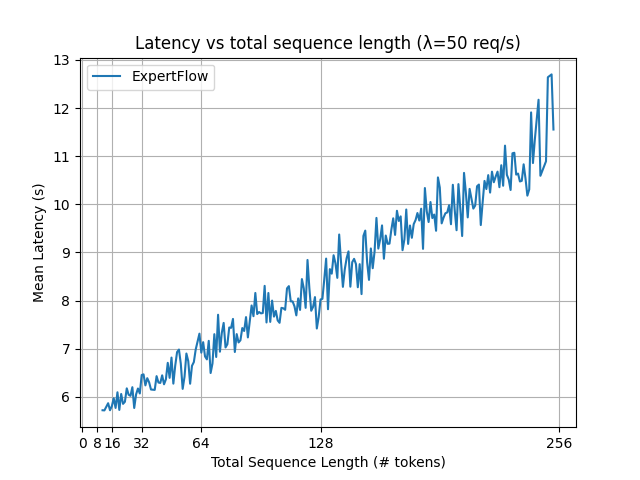
\includegraphics[width=0.6\linewidth]{figures/rate50.png}
    \caption{\textbf{The latency of serving a request as a function of the final request length} ($\lambda=50$ requests/second)}
    \label{fig:rate50}
\end{figure}

\begin{figure}[H]
    \centering
    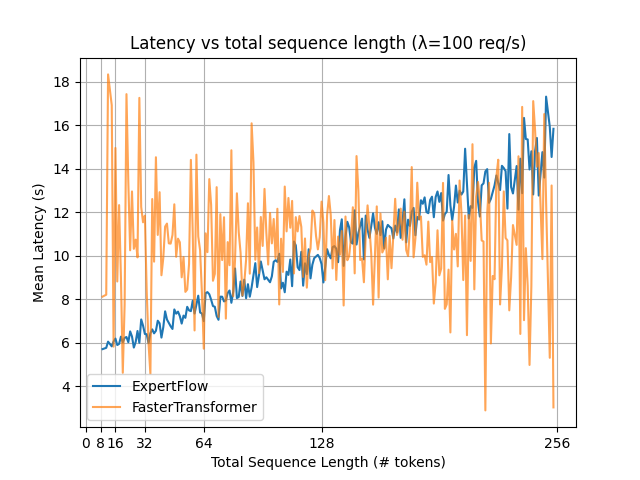
\includegraphics[width=0.6\linewidth]{figures/rate100.png}
    \caption{\textbf{The latency of serving a request as a function of the final request length} ($\lambda=100$ requests/second)}
    \label{fig:rate100}
\end{figure}

\begin{figure}[H]
    \centering
    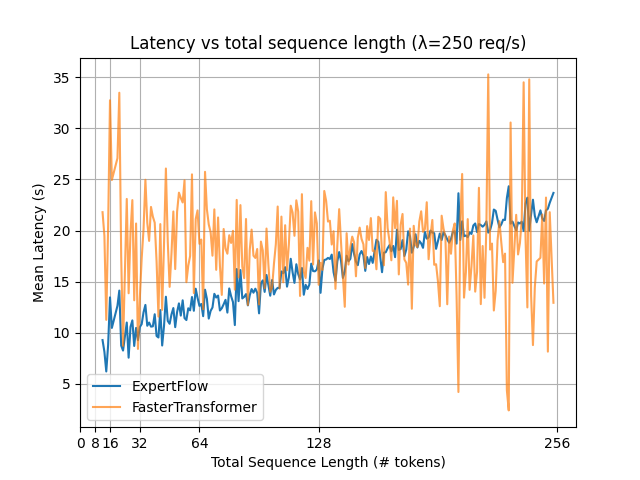
\includegraphics[width=0.6\linewidth]{figures/rate250.png}
    \caption{\textbf{The latency of serving a request as a function of the final request length} ($\lambda=250$ requests/second)}
    \label{fig:rate250}
\end{figure}

\begin{figure}[H]
    \centering
    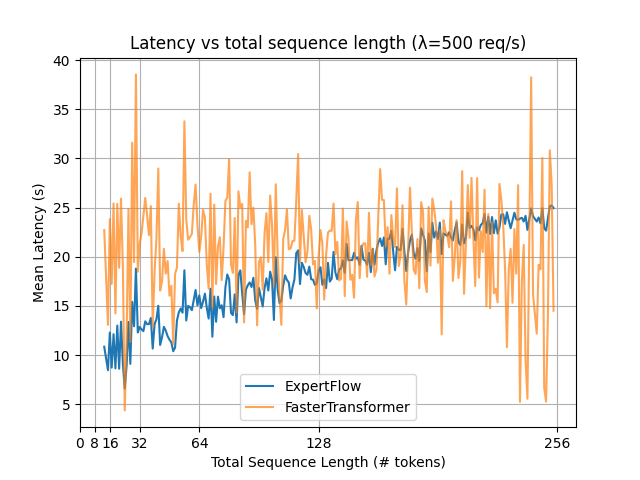
\includegraphics[width=0.6\linewidth]{figures/rate500.png}
    \caption{\textbf{The latency of serving a request as a function of the final request length} ($\lambda=500$ requests/second)}
    \label{fig:rate500}
\end{figure}

\subsubsection{Speculative Inference Evaluation}
We evaluate the performance of speculative inference by measuring the speedup compared to incremental decoding. We use 5 publicly-available prompt datasets, and first run the LLAMA-7B model in incremental decoding mode, measuring the execution time. Next, we repeat the experiment and use the LLAMA-7B model for token-tree verification, and use a set of speculators derived from LLAMA-160M. We observe speedups between 1.91x and 2.75x, as shown in Figure \ref{fig:latency}.

\begin{figure}
    \centering
    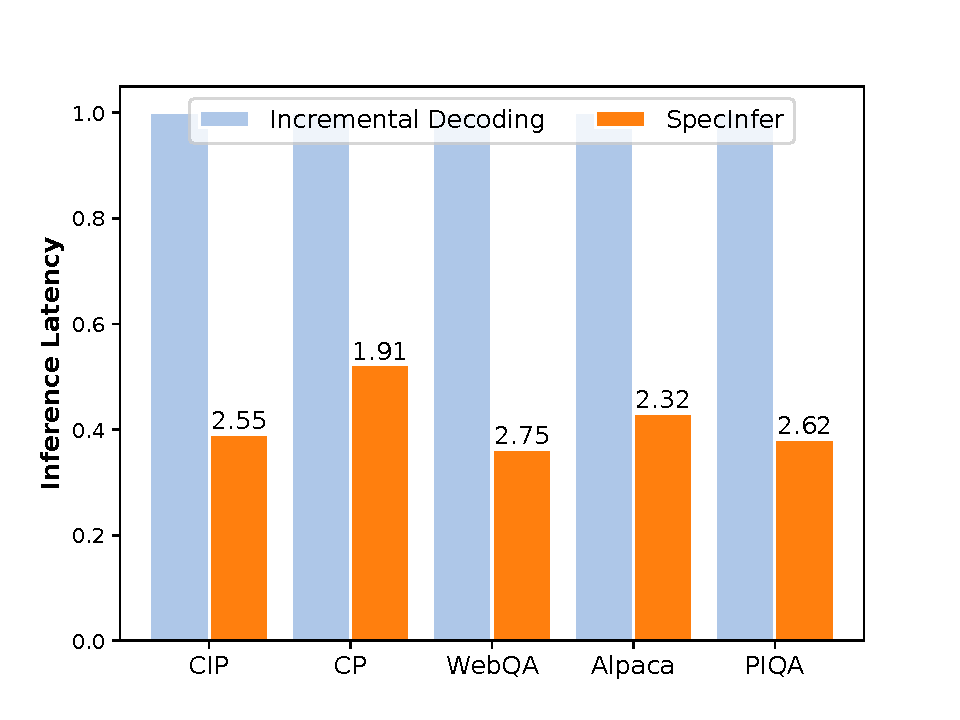
\includegraphics[scale=0.45]{figures/latency_improvement.pdf}
    \caption{\textbf{End-to-end inference latency speedup of speculative inference} when compared to incremental decoding, using five public prompt datasets. We use LLAMA-7B as the LLM and all SSMs are derived from LLAMA-160M}
    \label{fig:latency}
\end{figure}

\subsubsection{Future work}
Additional experiments could be useful to better understand the performance of ExpertFlow, the bottlenecks, and potential avenues for further improvement. Due to time constraints, we did not include these experiments in the current version of this document. Hence, we leave them to future work. Possible directions for additional evaluation efforts could be: an ablation study to evaluate the contribution of each of the system components towards the end-to-end performance; comparing our throughput and latency to DeepSpeed-MoE; running experiments under different sets of configurations. 

\section{Conclusion}
In this chapter, we described our efforts to evaluate the correctness and performance of ExpertFlow. In Section \ref{eval-correctness} we illustrated how we used unit and integration tests to ensure that our system can produce correct results, which align with other inference systems. In Section \ref{eval-performance}, we explained the setup for our experiments, and provided the results to measure the performance of ExpertFlow when compared to the baseline.
% !TeX root = ../thuthesis-example.tex

\chapter{Conclusion}\label{chapter-10}

\section{Summary}

\section{Limitations}

\section{Future Work}



% 其他部分
\backmatter

% 参考文献
\bibliography{ref/refs}  % 参考文献使用 BibTeX 编译
% \printbibliography       % 参考文献使用 BibLaTeX 编译

% 附录
% 本科生需要将附录放到声明之后,个人简历之前
\appendix
% % !TeX root = ../thuthesis-example.tex

\begin{survey}
\label{cha:survey}

\title{Title of the Survey}
\maketitle


\tableofcontents


本科生的外文资料调研阅读报告。


\section{Figures and Tables}

\subsection{Figures}

An example figure in appendix (Figure~\ref{fig:appendix-survey-figure}).

\begin{figure}
  \centering
  
\includegraphics[width=0.6\linewidth]{example-image-a.pdf}
  \caption{Example figure in appendix}
  \label{fig:appendix-survey-figure}
\end{figure}


\subsection{Tables}

An example table in appendix (Table~\ref{tab:appendix-survey-table}).

\begin{table}
  \centering
  \caption{Example table in appendix}
  \begin{tabular}{ll}
    \toprule
    File name       & Description                                         \\
    \midrule
    thuthesis.dtx   & The source file including documentaion and comments \\
    thuthesis.cls   & The template file                                   \\
    thuthesis-*.bst & BibTeX styles                                       \\
    thuthesis-*.bbx & BibLaTeX styles for bibliographies                  \\
    thuthesis-*.cbx & BibLaTeX styles for citations                       \\
    \bottomrule
  \end{tabular}
  \label{tab:appendix-survey-table}
\end{table}


\section{Equations}

An example equation in appendix (Equation~\eqref{eq:appendix-survey-equation}).
\begin{equation}
  \frac{1}{2 \uppi \symup{i}} \int_\gamma f = \sum_{k=1}^m n(\gamma; a_k) \mathscr{R}(f; a_k)
  \label{eq:appendix-survey-equation}
\end{equation}


\section{Citations}

Example citations in appendix.
\cite{abrahams99tex}
\cite{salomon1995advanced}
\cite{abrahams99tex,salomon1995advanced}


\bibliographystyle{unsrtnat}
\bibliography{ref/appendix}

\end{survey}
       % 本科生:外文资料的调研阅读报告
% % !TeX root = ../thuthesis-example.tex

\begin{translation}
\label{cha:translation}

\title{书面翻译题目}
\maketitle

\tableofcontents


本科生的外文资料书面翻译。


\section{图表示例}

\subsection{图}

附录中的图片示例(图~\ref{fig:appendix-translation-figure})。

\begin{figure}
  \centering
  
\includegraphics[width=0.6\linewidth]{example-image-a.pdf}
  \caption{附录中的图片示例}
  \label{fig:appendix-translation-figure}
\end{figure}


\subsection{表格}

附录中的表格示例(表~\ref{tab:appendix-translation-table})。

\begin{table}
  \centering
  \caption{附录中的表格示例}
  \begin{tabular}{ll}
    \toprule
    文件名          & 描述                         \\
    \midrule
    thuthesis.dtx   & 模板的源文件,包括文档和注释 \\
    thuthesis.cls   & 模板文件                     \\
    thuthesis-*.bst & BibTeX 参考文献表样式文件    \\
    thuthesis-*.bbx & BibLaTeX 参考文献表样式文件  \\
    thuthesis-*.cbx & BibLaTeX 引用样式文件        \\
    \bottomrule
  \end{tabular}
  \label{tab:appendix-translation-table}
\end{table}


\section{数学公式}

附录中的数学公式示例(公式\eqref{eq:appendix-translation-equation})。
\begin{equation}
  \frac{1}{2 \uppi \symup{i}} \int_\gamma f = \sum_{k=1}^m n(\gamma; a_k) \mathscr{R}(f; a_k)
  \label{eq:appendix-translation-equation}
\end{equation}


\section{文献引用}

文献引用示例\cite{abrahams99tex}。


\appendix

\section{附录}

附录的内容。


% 书面翻译的参考文献
\bibliographystyle{unsrtnat}
\bibliography{ref/appendix}

% 书面翻译对应的原文索引
\begin{translation-index}
  \nocite{salomon1995advanced}
  \bibliographystyle{unsrtnat}
  \bibliography{ref/appendix}
\end{translation-index}

\end{translation}
  % 本科生:外文资料的书面翻译
%% !TeX root = ../thuthesis-example.tex

\chapter{补充内容}

附录是与论文内容密切相关、但编入正文又影响整篇论文编排的条理和逻辑性的资料,例如某些重要的数据表格、计算程序、统计表等,是论文主体的补充内容,可根据需要设置。


\section{图表示例}

\subsection{图}

附录中的图片示例(图~\ref{fig:appendix-figure})。

\begin{figure}
  \centering
  
\includegraphics[width=0.6\linewidth]{example-image-a.pdf}
  \caption{附录中的图片示例}
  \label{fig:appendix-figure}
\end{figure}


\subsection{表格}

附录中的表格示例(表~\ref{tab:appendix-table})。

\begin{table}
  \centering
  \caption{附录中的表格示例}
  \begin{tabular}{ll}
    \toprule
    文件名          & 描述                         \\
    \midrule
    thuthesis.dtx   & 模板的源文件,包括文档和注释 \\
    thuthesis.cls   & 模板文件                     \\
    thuthesis-*.bst & BibTeX 参考文献表样式文件    \\
    thuthesis-*.bbx & BibLaTeX 参考文献表样式文件  \\
    thuthesis-*.cbx & BibLaTeX 引用样式文件        \\
    \bottomrule
  \end{tabular}
  \label{tab:appendix-table}
\end{table}


\section{数学公式}

附录中的数学公式示例(公式\eqref{eq:appendix-equation})。
\begin{equation}
  \frac{1}{2 \uppi \symup{i}} \int_\gamma f = \sum_{k=1}^m n(\gamma; a_k) \mathscr{R}(f; a_k)
  \label{eq:appendix-equation}
\end{equation}


% 致谢
% !TeX root = ../thuthesis-example.tex

\begin{acknowledgements}

First and foremost, I am deeply grateful to Prof. Jidong Zhai for his support and guidance throughout the entirety of this thesis project. From the proposal stage to the research process, final presentation, and revisions, Prof. Zhai's expertise and mentorship have been invaluable. Additionally, I am grateful for his feedback on my status reports and for his assistance in navigating the challenges posed by the border closure and my arrival at Tsinghua University, including helping me schedule meetings at times that worked in my timezone, and putting me in contact with fellow students that helped me understand and fill all required forms in time, despite knowing very little Chinese. I would also like to extend my heartfelt appreciation to Prof. Zhihao Jia from Carnegie Mellon University for co-advising the ExpertFlow project. His regular meetings, invaluable advice, and provision of necessary resources, including computing facilities for developing and testing the ExpertFlow prototype, have been immensely beneficial to my research progress. I am indebted to my Tsinghua classmates for their friendship and camaraderie, making me feel at home away from home. From online orientation events to working together on projects, meeting up in different cities like Paris and Milan, and finally being reunited on the beautiful Tsinghua campus in Beijing, these cherished memories have enriched my MS program experience. I am also grateful to my Tsinghua lab mates for their mentorship and assistance with my project, as well as helping me navigate campus life and having a unforgettable experience here at Tsinghua University. My heartfelt thanks also go to my CMU lab mates Daiyaan Arfeen, Xinhao Cheng, Zeyu Wang, Rae Wong, Zhihao Zhang, who have made significant contributions to the project, as well as to graduate students Reyna Abhyankar (UCSD) and Colin Unger (Stanford), who were involved extensively in the project. I would also like to recognize Xupeng Miao for helping me translate the title and abstract into Chinese. Finally, I am deeply grateful to my family, my girlfriend, and my friends for their unwavering love, support, and encouragement.

\end{acknowledgements}


% 声明
\statement
% 将签字扫描后的声明文件 scan-statement.pdf 替换原始页面
% \statement[file=scan-statement.pdf]
% 本科生编译生成的声明页默认不加页脚,插入扫描版时再补上;
% 研究生编译生成时有页眉页脚,插入扫描版时不再重复。
% 也可以手动控制是否加页眉页脚
% \statement[page-style=empty]
% \statement[file=scan-statement.pdf, page-style=plain]

% 个人简历、在学期间完成的相关学术成果
% 本科生可以附个人简历,也可以不附个人简历
% !TeX root = ../thuthesis-example.tex

\begin{resume}

  \section*{个人简历}

  Gabriele Oliaro was born on July 31, 1998 in Turin, Piedmont, Italy. He attended high school in Milan, Italy and graduated in 2017. He began his bachelor’s study in the School of Engineering and Applied Sciences, Harvard University, USA in August 2017, majoring in electrical engineering, and earned a Bachelor of Science degree in May 2021. He began his master’s study in the Department of Computer Science, Tsinghua University, China in September 2021, and is expected to earn a Master of Science degree in Computer Science in June 2023.


  \section*{在学期间完成的相关学术成果}

  \subsection*{学术论文}

  \begin{achievements}
    \item Langlet J., Ben-Basat R., Ramanathan S., Oliaro G., Mitzenmacher M., Yu M., Antichi G. 2021. Zero-CPU Collection with Direct Telemetry Access. ACM Workshop on Hot Topics in Networks 2021 (HotNets '21). https://doi.org/10.1145/3484266.3487366
    \item Oliaro G. Pitcher: A Probabilistic In-band Telemetry Checker. Bachelor Thesis. Harvard University, 2021.
  \end{achievements}


  \subsection*{预印本}

  \begin{achievements}
    \item Langlet J., Ben-Basat R., Ramanathan S., Oliaro G., Mitzenmacher M., Yu M., Antichi G. 2022. Direct Telemetry Access. Arxiv Preprint. https://doi.org/10.48550/arXiv.2202.02270
  \end{achievements}

\end{resume}


% 指导教师/指导小组评语
% 本科生不需要
% !TeX root = ../thuthesis-example.tex

\begin{comments}
% \begin{comments}[name = {指导小组评语}]
% \begin{comments}[name = {Comments from Thesis Supervisor}]
% \begin{comments}[name = {Comments from Thesis Supervision Committee}]

  论文提出了……

\end{comments}


% 答辩委员会决议书
% 本科生不需要
% !TeX root = ../thuthesis-example.tex

\begin{resolution}

  The resolution will go here

\end{resolution}


% 本科生的综合论文训练记录表(扫描版)
% \record{file=scan-record.pdf}

\end{document}
